\documentclass[10pt,twocolumn,letterpaper]{article}

\usepackage{cvpr}
\usepackage{times}
\usepackage{epsfig}
\usepackage{graphicx}
\usepackage{amsmath}
\usepackage{amssymb}
\usepackage{appendix}

% Include other packages here, before hyperref.

% for using the same institution for all three authors
\usepackage{authblk}
% for the ä in Universität
\usepackage[utf8]{inputenc}

\usepackage{subcaption}

% tables
\usepackage{booktabs}
\usepackage{multirow}
\usepackage{nicefrac}

% If you comment hyperref and then uncomment it, you should delete
% egpaper.aux before re-running latex.  (Or just hit 'q' on the first latex
% run, let it finish, and you should be clear).
\usepackage[pagebackref=true,breaklinks=true,letterpaper=true,colorlinks,bookmarks=false]{hyperref}
\usepackage{xargs}                      % Use more than one optional parameter in a new commands
\usepackage[pdftex,dvipsnames]{xcolor}  % Coloured text etc.
\usepackage[colorinlistoftodos,textsize=small]{todonotes}
\newcommandx{\todoc}[2][1=]{\todo[linecolor=orange,backgroundcolor=orange!25,bordercolor=orange,#1]{TODO: #2}}
\newcommandx{\unsure}[2][1=]{\todo[linecolor=red,backgroundcolor=red!25,bordercolor=red,#1]{UNSURE: #2}}
\newcommandx{\change}[2][1=]{\todo[linecolor=blue,backgroundcolor=blue!25,bordercolor=blue,#1]{CHANGE: #2}}
\newcommandx{\info}[2][1=]{\todo[linecolor=OliveGreen,backgroundcolor=OliveGreen!25,bordercolor=OliveGreen,#1]{INFO: #2}}
\newcommandx{\improvement}[2][1=]{\todo[linecolor=Plum,backgroundcolor=Plum!25,bordercolor=Plum,#1]{IMPROVEMENT: #2}}
\newcommandx{\thiswillnotshow}[2][1=]{\todo[disable,#1]{THIS WILL NOT SHOW: #2}}
\setlength{\marginparwidth}{2cm}

\cvprfinalcopy % *** Uncomment this line for the final submission

\def\cvprPaperID{****} % *** Enter the CVPR Paper ID here
\def\httilde{\mbox{\tt\raisebox{-.5ex}{\symbol{126}}}}

% Pages are numbered in submission mode, and unnumbered in camera-ready
% The following line needs to be commented out if one wants page-number in final publication mode
%\ifcvprfinal\pagestyle{empty}\fi
\begin{document}

%%%%%%%%% TITLE
\title{Unsupervised Monocular Depth Estimation Using Atrous Convolutions}

\author{Fabian Kessler}
\author{Steven Lang}
\author{Dominik Straub}

\affil{Technische Universität Darmstadt \authorcr
  \{\tt firstname.lastname\}@stud.tu-darmstadt.de}

\maketitle
%\thispagestyle{empty}
%%%%%%%%% ABSTRACT
\begin{abstract}
Monocular depth estimation is concerned with computing a dense depth map from a single image but faces difficulties especially at object boundaries.
Atrous convolutions have been successfully employed to this end in the task of semantic segmentation.
In this paper, we investigate, whether it is  also possible to apply atrous convolutions in unsupervised monocular depth estimation. 
Specifically, we place an Atrous Spatial Pyramid Pooling block in a convolutional neural network between the encoder and decoder. 
This block allows for computing feature maps at different spatial scales on top of the encoder output. 
Our experiments show that atrous convolutions in the proposed setup do not improve depth estimation performance. 
Furthermore, the necessity of a lower output stride after the encoder, such that an increased receptive field size is even applicable, harms runtime and increases memory consumption. 
Finally, we show that it is possible to reduce the number of channels after the encoder, which reduces the parameter count without impairing predictions.
\end{abstract}
%%%%%%%%% BODY TEXT
%%%%%%%%% INTRO
\section{Introduction}
Depth estimation is one of the most researched areas in computer vision.
While traditionally sparse stereo correspondence algorithms were used, most modern work is concerned with estimating dense depth maps from images.
Typically, this is achieved via a stereo matching approach, in which (under certain assumptions about epipolar geometry and the appearance of surfaces) a disparity map can be computed by warping one image of a stereo  pair into the other.
As described by Scharstein \& Szeliski~\cite{scharstein2002taxonomy}, this usually involves an appearance cost function, a global smoothness constraint and iterative refinements of depth maps.
Most contemporary approaches still make use of these basic ingredients.

Stereo-based approaches have the inherent disadvantages that they require a stereo image pair for each newly generated depth estimate.
The respective stereo data, however, is not available for the majority of use-cases.
This has sparked research into monocular depth estimation methods, which are usually based on machine learning models trained on large amounts of ground truth depth data.
Ground truth depth data, however, is very tedious to capture. 
It requires the use of expensive and finely calibrated depth scanning hardware such as LiDAR sensors. These introduce further problems including noise in distant samples, sparse measuring, as well as sensor calibration difficulties. Therefore, ground truth depth data is not available in large quantities for most scenarios.
The KITTI Stereo dataset from 2015 for example\cite{Menze2015CVPR}, consisting of only 200 images, was captured using a LiDAR sensor and consequently, depth is only available for about 5\% of the pixels and only for non-moving objects. 

Because of this, recent monocular depth estimation methods~\cite{garg2016unsupervised,Godard_2017_CVPR,Godard2018} approach the estimation process as an unsupervised image reconstruction problem, in which stereo or video data is only required during training and can easily be captured with modern smartphones, for example. 
The monocular depth estimation architecture by Godard \etal~\cite{Godard_2017_CVPR} demonstrated that when enforcing consistency between two predicted depth maps and the two camera views, superior performance to fully-supervised baselines and generalization to yet unseen datasets can be achieved.
Most of their depth estimates' uncertainty can be found in uniform regions and at object boundaries. 

This is not surprising, since dense predictions tasks, such as semantic segmentation and depth estimation, face two key challenges: Capturing rich contextual information and detecting objects at multiple scales, while also maintaining sharp object boundaries in the final dense prediction.
State of the art CNN architectures typically use small filter sizes, repeated striding operations and max-pooling to down-sample the image, which reduce the resolution of feature maps and as a result make details difficult to recover.
As mentioned by Fu \etal~\cite{Fu2018}, previous solutions include the use of skip-connections~\cite{Ronneberger2015}, iterative refinement or multi-layer deconvolution networks~\cite{noh2015learning}. 
\begin{figure}
    \centering
    \begin{subfigure}[b]{0.35\linewidth}
    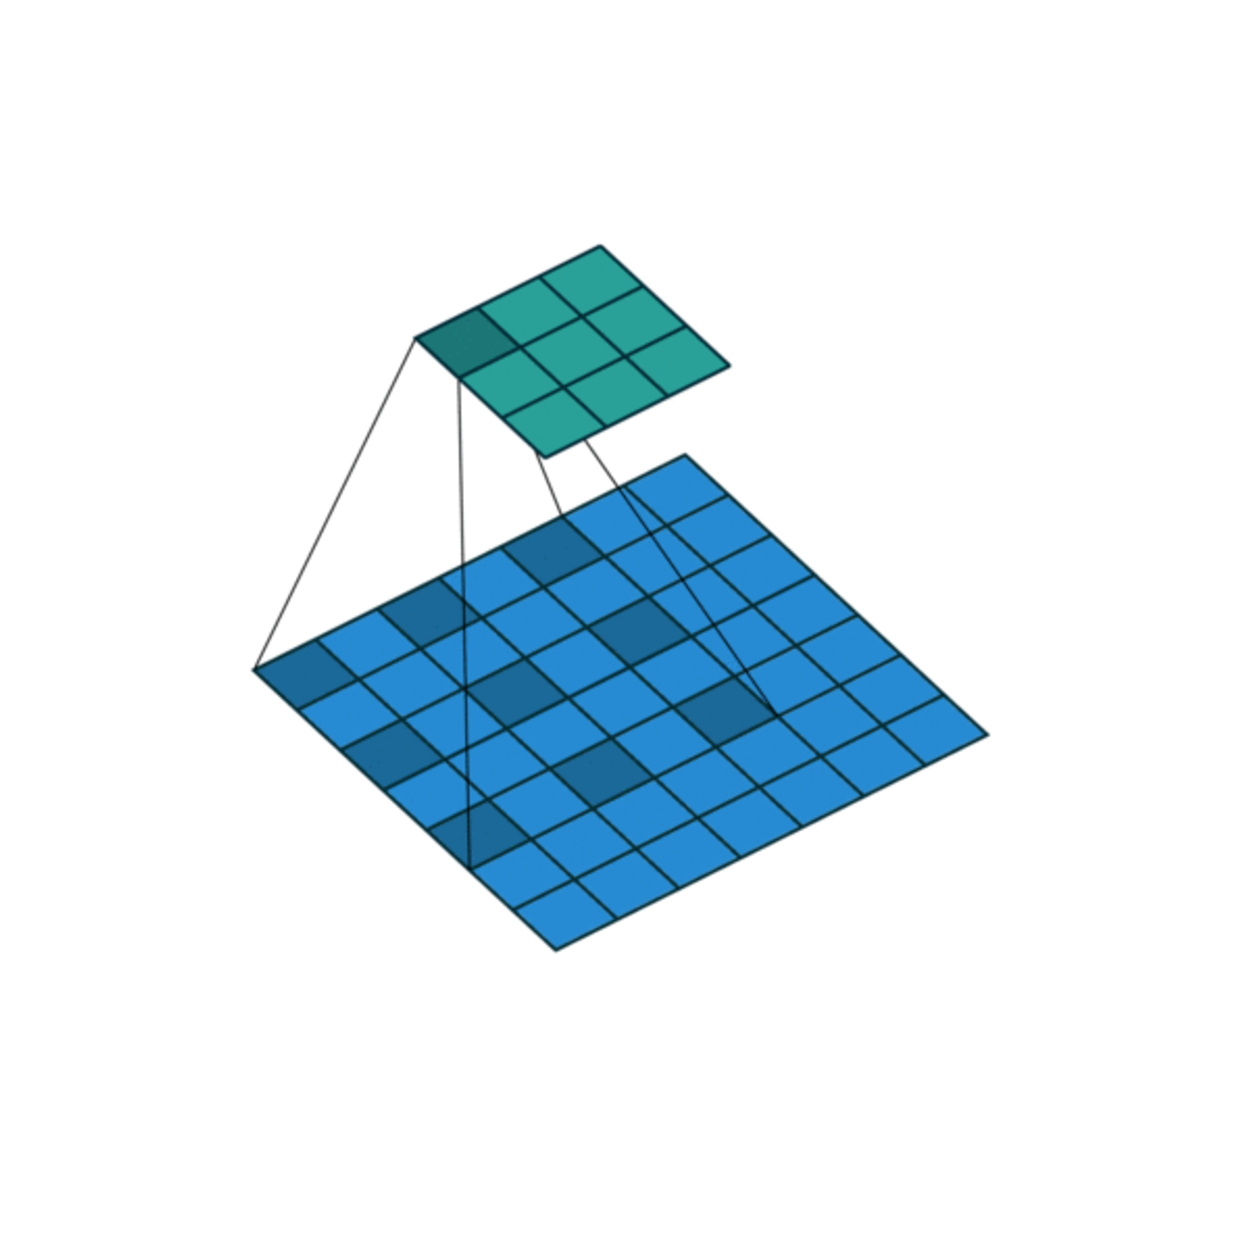
\includegraphics[width=1.0\linewidth]{images/concepts/dilation.pdf}
    \caption{}
    \label{fig:atrous-convolution}
    \end{subfigure}
    \begin{subfigure}[b]{0.6\linewidth}
        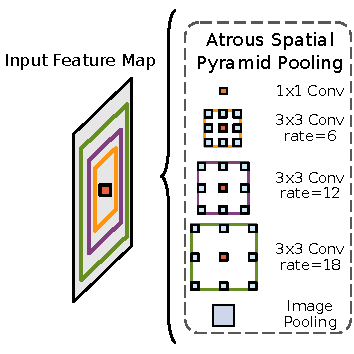
\includegraphics[width=1.0\linewidth]{images/architecture/aspp.pdf}
        \caption{}
        \label{fig:aspp}
    \end{subfigure}
    \caption{(a) Atrous convolution with a dilation rate of 2. (b) Atrous Spatial Pyramid Pooling (ASPP). The field of views of the different atrous convolutions are shown in different colors on the input feature map. Figure adapted from Chen \etal~\cite{chen2018deeplab}.}
\end{figure}

In this work, we investigate whether atrous convolutions, which have proven successful in semantic segmentation~\cite{chen2018deeplab, chen2018encoder}, can also improve monocular depth estimation.
Atrous convolutions allow to explicitly control the receptive field size of a filter without introducing additional parameters.
This is achieved by skipping pixels at a certain rate (also called filter dilation), and thus inserting zero holes (french: \textit{trous}) into the filter (see \figurename~\ref{fig:atrous-convolution}).
This helps with aggregating information from different spatial scales, while also allowing for larger feature maps, as less downsampling is required in order to achieve a large field of view (FOV). 

With these considerations in mind, we designed an architecture using atrous convolutions based on the original monocular depth estimation architecture from Godard \etal~\cite{Godard_2017_CVPR}, and we compare this both visually and quantitatively to the original baseline. In the architecture design, we considered predictive performance and runtime and memory consumption.
We performed several experiments that show how these factors are influenced by different architectural decisions.
We conclude that atrous convolutions, at least in the setups we investigated, do not improve monocular depth estimation. 
Based on our experiments we propose an architecture that improves upon the baseline performance from Gordard \etal~\cite{Godard_2017_CVPR} while cutting the number of parameters by 24.5\%. 



%%%%%%%%% RELATED WORK
\section{Related Work}
Depth estimation can either be performed on stereo or monocular images, the latter being a more challenging problem. Stereo-based approaches have a long history in computer vision, ranging from more classical methods~\cite{scharstein2002taxonomy} to recent advancements in deep learning~\cite{zbontar2016stereo}.
In this work, we are concerned with monocular depth estimation, where only a single input image is available at test time.

\subsection{Monocular Depth Estimation}
We give an overview of the two main approaches for monocular depth estimation: supervised methods, which use ground truth depth data, and unsupervised methods, typically using image pairs during training. 

\subsubsection{Supervised Approaches}

Early approaches of monocular depth estimation were based on segmenting images into superpixel patches and then inferring the 3D position and orientation of these patches based on geometric and image-formation assumptions~\cite{saxena2009make3d, Lin2012}. Most of these methods relied on the use of hand-crafted feature representations such as SIFT~\cite{Lin2010}.

Modern Deep Convolutional Neural Networks (CNN) allow representing the data using richer features that are learned within the network for a specific task.
Eigen \etal~\cite{eigen2015predicting, eigen2014depth} was the first to propose monocular depth estimation as a CNN-based pixel-wise continuous regression problem in order to obtain depth.
This work also highlights the importance of multi-scale features, by employing two networks to learn both the global scene structure, along with a second network to refine the depth prediction based on more local features (e.g. walls and objects).  

Since then several ideas have been proposed to improve upon the results of a pixel-based regression approach, including the use of multi-scale continuous conditional random fields~\cite{DBLP:journals/corr/abs-1803-00891}, semantic information~\cite{ramirez2018}, attention~\cite{Jiao2018,Chen2019} or edge-specific loss-terms~\cite{Hu2018}. 
Jiao \etal~\cite{Jiao2018} employ semantic information, in addition to an attention-based loss term that gives higher weight to more distant regions. 
This setup improves the accuracy of distant depth estimates, as depth estimation networks can suffer from being ``short-sighted'', due to closer distances being over-represented in the loss. 
The quality of depth predictions at object boundaries can be improved by fusing information from different spatial scales (multi-scale feature fusion) and employing edge-specific loss-functions using both differences in gradients and angle of surface normals between the estimated depth maps and the corresponding ground truths data~\cite{Hu2018}. 
Alternatively, monocular depth estimation can also be formulated as pixel-wise classification~\cite{Cao2018} or ordinal regression~\cite{Fu2018}. In this approach, the ranges of possible depths are learned instead of exact depth values. These depth ranges are easier to estimate and allow to reason about the confidence of the predictions and can even lead to superior performance. 

\subsubsection{Unsupervised Approaches}

Unsupervised methods provide an alternative to the supervised methods, in so far that they do not need labeled ground truth depth data, which is not widely available for many application domains and datasets.
Instead, these methods rely on estimating disparity maps from either rectified stereo pairs~\cite{garg2016unsupervised,Godard_2017_CVPR} or sequences of videos~\cite{Wang2017,Godard2018} by learning a mapping between images that correspond to depth or disparity. Importantly, the image pairs are only available during training, which makes the methods monocular at test time.
Garg \etal~\cite{garg2016unsupervised} suggested directly learning a disparity map through an encoder-decoder CNN, by applying a photo-metric difference loss to compare the reconstructed image, to the true target image.
This approach was further refined by Godard \etal~\cite{Godard_2017_CVPR} through learning two disparity maps instead of one and enforcing consistency between both maps, along with the reconstructed images and their respective input images. 

More recent work has focused on the use of video data to solve depth estimation by performing view-synthesis based on successive frames~\cite{Wang2017,Casser2018,Godard2018}.
Typically, this involves training a separate pose network to learn the corresponding camera transformations and depth information.
Recent work by Godard \etal~\cite{Godard2018} shows that depth features can also help in pose estimation, by sharing weights between the two networks.  
One drawback of video-based approaches is that they can not effectively deal with moving objects between frames.
Objects moving together with the camera are typically projected into infinite depth, such that the photo-metric loss is lowered.
A recent approach~\cite{Casser2018} has shown that it is possible to explicitly model and account for individual object motion by obtaining both their speed and direction and warping them independent of background motion.
This can lead to performance comparable to stereo-based approaches.
Gordard \etal~\cite{Godard2018} showed, that the network can be trained with both monocular, as well as stereo data to overcome this problem and achieve state-of-the-art performance.

Furthermore, semi-supervised approaches have been suggested in which both the ground truth depth data, along with the image data is used to ensure image-consistency of the depth maps and correspondence to the ground truth depth~\cite{DBLP:journals/corr/KuznietsovSL17}. 

\subsection{Atrous Convolutions}

%Argument for why to use Atrous Convolutions 

Atrous convolutions were originally introduced in the context of wavelet transforms~\cite{holschneider1990wavelet} as a means of reducing computational complexity. Since atrous convolutions skip certain pixels, they achieve a larger filter without the need for additional parameters.
Recently, atrous convolutions have been heavily used in semantic segmentation~\cite{chen2018deeplab, chen2018encoder, wang2018understanding, YuKoltun2016}, with some applications to other tasks such as image classification~\cite{Yu_2017_CVPR}.
When depth estimation is treated as a classification task, recent work suggests that atrous convolutions can also be successfully employed to obtain feature maps at different spatial scales without repeated downsampling of the image~\cite{Fu2018,Chen2019}. 
Inspired by these successful applications, we apply atrous convolutions to monocular depth estimation as a regression problem.


%%%%%%%%% METHODS
\section{Methods}
\label{sec:methods}
In this section, we briefly describe the approach by Godard \etal~\cite{Godard_2017_CVPR}.
We then explain atrous convolutions and how we extended Godard \etal's architecture with atrous convolutions.

\subsection{Monocular Depth Estimation}
\label{sec:methods:depth-estimation}
Monocular depth estimation can be treated as a stereo reconstruction problem, where a left an right image ($I^l$ and $I^r$) are available during training.
The left image is fed through an encoder-decoder CNN, which outputs a disparity map w.r.t. the right image ($d^r$).
\begin{figure}
    \centering
    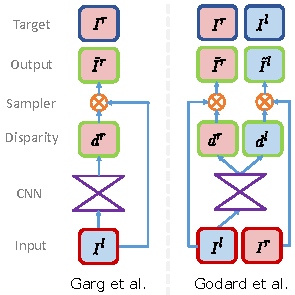
\includegraphics[width=0.8\linewidth]{images/architecture/monodepth.pdf}
    \caption{Monocular depth estimation via stereo reconstruction: naive approach by Garg et al.~\cite{garg2016unsupervised} and method with left-right consistency (figure adapted from Godard et al.~\cite{Godard_2017_CVPR}).}
    \label{fig:monodepth}
\end{figure}
This disparity map is applied to the left image using backward warping with bilinear interpolation in order to obtain the reconstructed right image $\Tilde{I}^r$ (see \figurename~\ref{fig:monodepth}, left column).
The CNN can be trained with an appearance-based loss function that measures the photometric difference between $I^r$ and $\Tilde{I}^r$.

Godard \etal's~\cite{Godard_2017_CVPR} main contribution is the idea of left-right consistency: instead generating only the right disparity map, the CNN outputs a pair of corresponding left and right disparity maps ($d^l$ and $d^r$).
The left image is further warped with the right disparity map and vice versa (see \figurename~\ref{fig:monodepth}, right column).
The loss function consists of three weighted terms:
\begin{align}
    C_s = \alpha_{ap}C_{ap} + \alpha_{ds}C_{ds} + \alpha_{lr}C_{lr} \quad .
\end{align}
$C_{ap}$ is the appearance-based loss, $C_{ds}$ is a disparity smoothness term, which penalizes high derivatives in the disparity maps, and $C_{lr}$ is a left-right consistency penalty, which ensures that the left and right disparity maps agree.
Each term is weighted with an $\alpha$ value respectively.
Additionally, this loss is computed and summed across four different output scales: $C = \sum_{s=1}^4 C_s$.

We use these basic ideas (image reconstruction, smoothness, left-right consistency), but instead of a standard ResNet50 backbone, we experiment with atrous convolutions.


\subsection{Atrous Convolutions}
The output $g(i)$ at index  $i$ of a 1D atrous convolution $w$ is given by
\begin{align}
    g(i) = \sum_{k=1}^K x(i + rk) w(k) \quad ,
\end{align}
where $x$ is the input and $K$ is the filter size. The filter dilation $r$ specifies the rate at which the input is sampled. A standard convolution is a special case of an atrous convolution, where $r = 1$. 
The notion of an atrous convolution can be generalized to 2D for vision problems straightforward. \figurename~\ref{fig:atrous-convolution} shows a 2D atrous convolution with $r=2$.

We employ the idea of an Atrous Spatial Pyramid Pooling (ASPP) block~\cite{chen2018deeplab}, which contains several atrous convolutions with different atrous rates in parallel (see \figurename~\ref{fig:aspp}).
This is motivated by classical image pyramid methods~\cite{Witkin1987,quam1987hierarchical}, which process images at different spatial scales. 
Since varying atrous rates results in filters of different spatial dimensions, an ASPP block resembles a feature map at different spatial scales.
The atrous convolutions, along with a global averaging pooling layer, are concatenated and passed through a $1 \times 1$ convolution, which reduces the number of channels to 256.

\subsection{Output Stride}
\begin{figure}
    \centering
    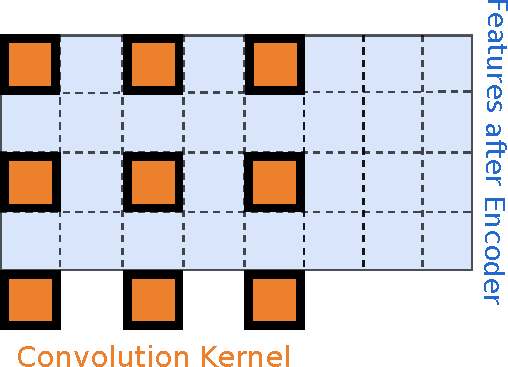
\includegraphics[width=0.6\linewidth]{images/architecture/os64-atrous-conv-with-text.pdf}
    \caption{A $4 \times 8$ feature map processed with an atrous convolution with rate 2.
    Some of the filter weights are out of the image range, which results in boundary issues.
    This effect is even stronger for convolutions with larger atrous rates.}
    \label{fig:output-stride}
\end{figure}
The output stride of a feature map is the factor by which its spatial dimensions are smaller than those of the input image.
Each ResNet block changes the output stride by a factor determined by the stride of its main convolutional layer.
In a standard ResNet50, each ResNet block has a stride of 2, which yields an output stride of 64 after the encoder.
This was also used in the monocular depth estimation architecture by Godard \etal, resulting in a $4\times8$ feature map after the encoder for $256 \times 512$ input images.
But in order to obtain feature responses at different spatial scales using atrous convolutions (with varying kernel size and thus FOVs), a certain size of image is required as illustrated in \figurename~\ref{fig:output-stride}.
Hence, we made the output stride in our network architecture variable by adapting the ResNet block output strieds.

\subsection{Our Architecture}
\begin{figure*}
\begin{center}
    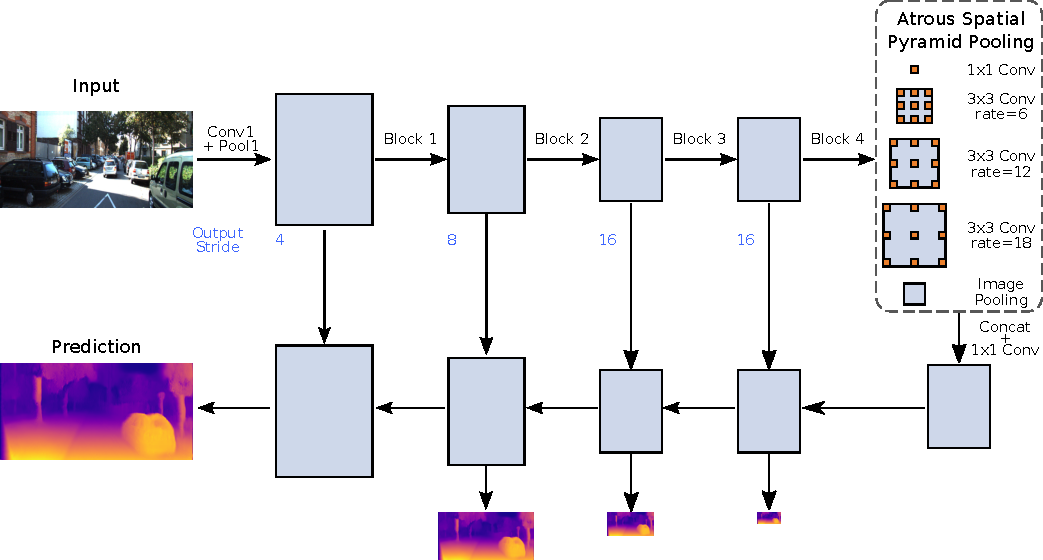
\includegraphics[width=0.9\linewidth]{images/architecture/architecture.pdf}
\end{center}
    \caption{Overview of our architecture.
    The input image is fed through a ResNet50 architecture, consisting of four blocks.
    Final feature maps of ResNet50 are passed to the ASPP block, which processes its input at several spatial scales in parallel.
    The decoder then upsamples the image again, while taking low-level features from the skip-connections and outputting disparity maps at multiple spatial scales.}
    \label{fig:our_architecture}
\label{fig:short}
\end{figure*}
\figurename~\ref{fig:our_architecture} shows a sketch of our architecture.
We use the same basic setup as Godard \etal~\cite{Godard_2017_CVPR}, i.e. a ResNet50 backbone, skip connections between the encoder and the decoder and output disparities at multiple spatial scales.
Our main contribution is the extension of the encoder by an ASPP block, inspired by the DeepLab architecture~\cite{chen2018deeplab}. For our main experiments, we insert the ASPP module after the final layer of the ResNet50, since this placement has proven to work well in other work~\cite{chen2018encoder, Fu2018}. Alternative choices, e.g. in between ResNet blocks, are also possible (see Section \ref{section:experiments:atrous-encoder} and supplement \ref{appendix:atrous-encoder}).

The ASPP block introduces additional parameters to the architecture.
By processing the ASPP block output with a $1\times 1$ convolution, we reduce the number of feature maps to 256 after the encoder, compared to 2048 feature maps in the original architecture.
Since this reduces the decoder input dimensionality, we effectively keep the number of parameters identical to the original architecture at 58.4 million\footnote{While inspecting the TensorFlow implementation by Godard \etal, we found that their ResNet50-based architecture, in fact, had 58.4 million parameters, instead of the specified 48 million.}.






%%%%%%%%% RESULTS
\section{Results}
\label{section:experiments}

The encoder-decoder network was implemented using PyTorch~\cite{paszke2017automatic} (version \texttt{1.0.1}) and training took place on a single GPU (NVIDIA GeForce GTX 1080 Ti or GTX TITAN X).
For all our experiments we used the KITTI data set~\cite{Geiger2013IJRR} with a total number of 30159 images from which 29000 were used during training and 1159 for validation. Additionally, the KITTI Stereo 2015 dataset~\cite{Menze2015CVPR} provided 200 ground truth disparities which were used for numerical comparisons between models. This evaluation was performed by converting both, the predicted disparities, as well as the sparse ground truth disparities into depth space and capping depth to 80 meters.

We used metrics for numerical evaluation found in Eigen \etal~\cite{eigen2014depth} and present the absolute relative error for our experiments. A table with all metrics for all experiments can be found in Supplement \ref{appendix:full-results}. Additionally, to bring the results of the following sections into perspective, we repeated the baseline implementation 12 times with different random seeds and measured the mean and standard deviation of the error metrics. For the abs. rel. error e.g., we observed a mean of $0.1125$ and a standard deviation of $8.581 \times 10^{-4}$. We also noticed about 25\% of the runs were not able to learn, with the loss staying constant at the initial value. Thus the networks performance was not robust to weight initialization.

Most of the training parameters were adopted from Godard \etal, including the number of epochs, learning-rate, optimization procedure, and data augmentation.
Specifically we trained our network for 50 epochs using the Adam optimizer~\cite{kingma2014adam} ($\beta_1 = 0.9, \beta_2 = 0.999$ and $\epsilon = 10^{-8} $). The initial learning rate of $\lambda = 10^{-4}$ was adjusted according to the batch size (i.e. doubling the learning rate when doubling the batch size).
Separate experiments confirmed that batch size did not affect training results significantly when also doubling the learning rate, hence we decided to use a batch size of 16 and thus $\lambda = 2*10^{-4}$ for our initial learning rate. This learning rate stayed constant for the first 30 epochs of training and was then halved every 10 epochs for the rest of the training. The training duration was 20 hours on average and mostly depended on the GPU and the output stride.
Values for the loss weight hyperparameters $\alpha$ from Section~\ref{sec:methods:depth-estimation} were inherited from the original paper. For these, no further hyperparameter optimizations have been conducted.

For training, the KITTI images were resized from $1275\times375$ to $512\times256$ and the same data augmentation as in the original paper was performed. This included flipping both images horizontally at $50\%$ chance level, as well as uniformly distributed gamma [0.8,1.2], brightness [0.5,2.0] and color shifts [0.8,1.2]. 

% TODO: cityscapes pretraining
For our final selection of models, we also employed cityscapes~\cite{Cordts2016Cityscapes} pretraining, followed by fine-tuning on KITTI. Here we used the same learning-rate and epoch count for both pretraining and fine-tuning.

\subsection{Baseline: Implementation Issues}
\label{sec:experiments:baseline}
Before running experiments with architectural changes, we replicated the original publication's~\cite{Godard_2017_CVPR} results. During this process, we encountered some difficulties:
\begin{figure}[t]
    \centering
    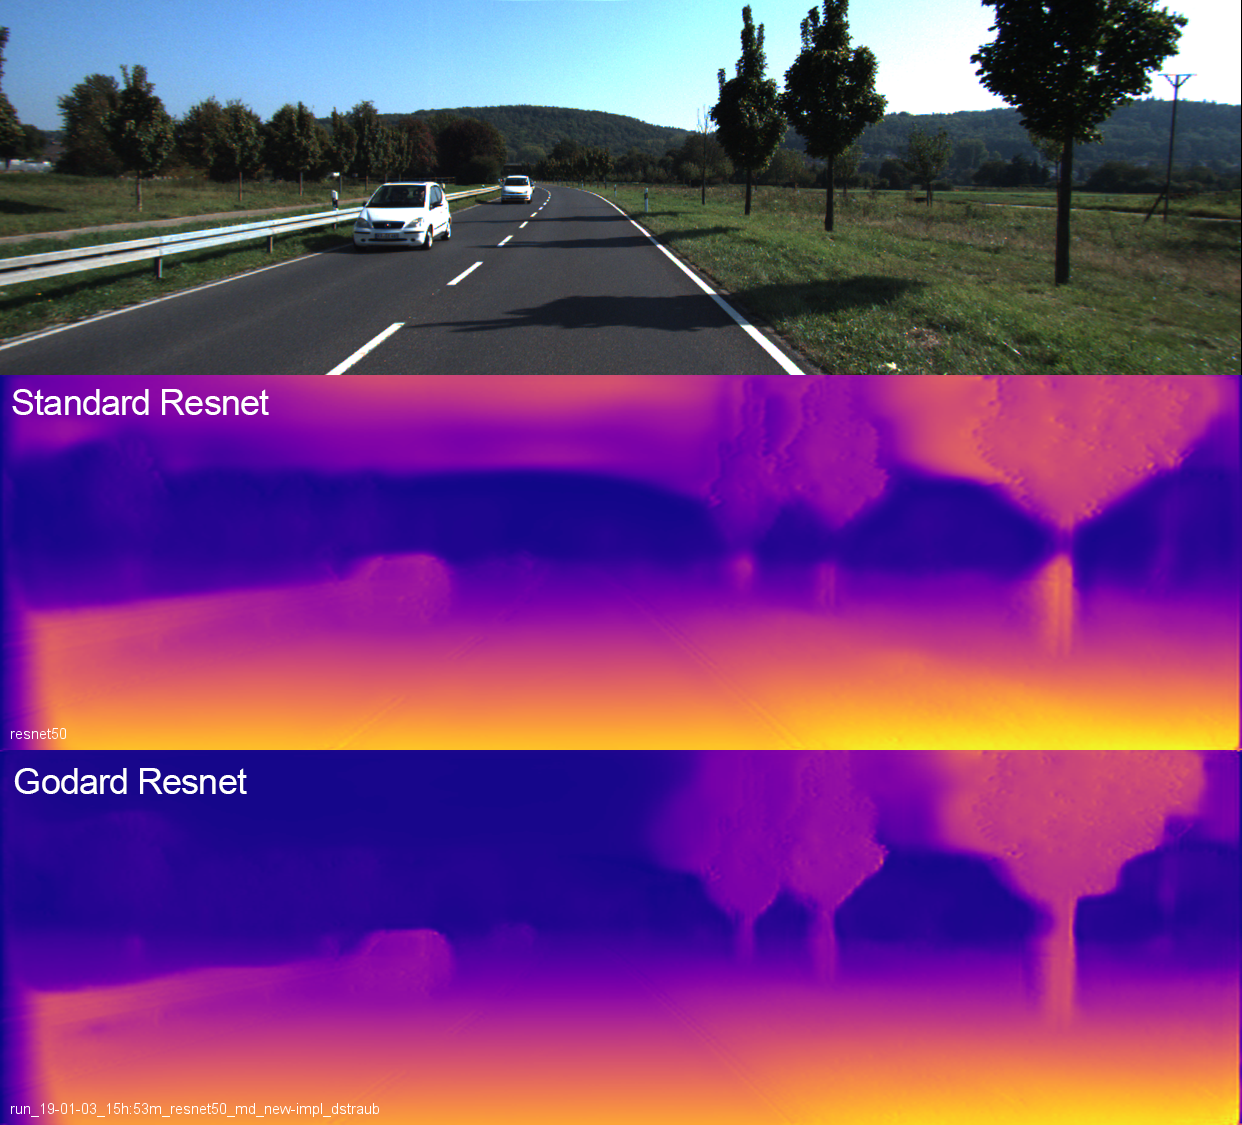
\includegraphics[width=0.8\linewidth]{images/disparities/implementationcomparison_001.png}
    \caption{Comparison between a standard ResNet50 and Godard \etal's ResNet50. Disparities from a standard ResNet50 show severe artifacts in the uniform sky regions, while the modified ResNet50 does not exhibit these problems.}
    \label{fig:sky_artifacts}
\end{figure}
Using the standard ResNet50 architecture from the PyTorch package as the encoder resulted in vastly underestimated depth in the uniform sky regions of the KITTI dataset (see \figurename~\ref{fig:sky_artifacts}, middle row).
This was not present in the disparity maps provided by the original authors~\cite{Godard_2017_CVPR}, which prompted us to investigate Godard \etal's ResNet50 implementation more thoroughly.
We found the following three differences between their implementation compared to a standard ResNet50: 
1) Lack of batch normalization,
2) using nearest neighbor instead of linear upsampling in the decoder and 
3) switching the order of convolutions with \textit{stride} $=1$ and \textit{stride} $= 2$ inside a ResNet block. 
While these differences were tested in isolation, we could not figure out which caused the different behavior of the networks.
However, porting the original TensorFlow implementation line by line to PyTorch fixed the erroneous estimations in homogeneous regions, such as the sky (see \figurename~\ref{fig:sky_artifacts}, bottom row).
Therefore, we used the modified ResNet50 implementation in all following experiments.

\subsection{Output Stride}
\label{section:experiments:output-stride}

\begin{table}

\begin{tabular}{rrrrr}
\toprule
Stride &  Abs. Rel. & Runtime {\tiny $\left(\frac{Min.}{Epoch}\right)$} & Memory (GB) & Param. (M) \\
\midrule
64 &    0.1120 & \textbf{15}  &     \textbf{6.12} &  58.4 \\
32 &    0.1048 &  29  &     8.87 &  58.4 \\
16 &    \textbf{0.1041} &  29  &     8.88 &  58.4 \\
8 &     0.1068 &  43  &    10.61 &  58.4 \\
\bottomrule
\end{tabular}

\caption{Baseline model~\cite{Godard_2017_CVPR} with different output strides (64 being the default): the absolute relative error is optimal at an output stride of 16, while the runtime and memory consumption monotonically increase when decreasing the output stride.}
\label{table:outstride}
\end{table}
Since atrous convolutions can only be effective for images of a certain resolution, which allows the whole kernel to be inside the image, we needed to decrease the output stride of the network (i.e. increase the input size to the ASPP). We conducted an experiment with varying output strides in the baseline model in order to isolate the output stride effect, such that the effect of the ASPP is really due to the ASPP and not merely due to the decreased output stride.
We tested four different output strides (namely 8, 16, 32 and 64) for their effect on predictions and computation time required per epoch.
The results in \tablename~\ref{table:outstride} show that increasing the output stride up to 16 decreases the abs. rel. error on the evaluation, while increasing the training time required for one epoch.
The abs. rel. error increased for output stride 8, among a substantially longer training time.
Unless otherwise specified, we focused on output stride 32 for the following experiments, as this provided the best trade-off between prediction performance and computation time. 

\subsection{ASPP Rates}
\label{section:aspp-rates}
\begin{figure}[t]
    \begin{center}
       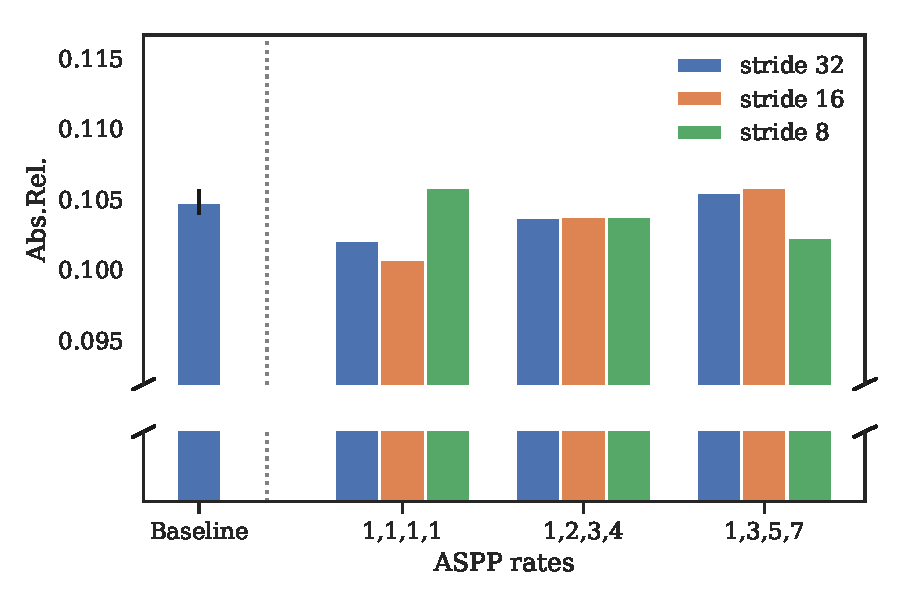
\includegraphics[width=1.0\linewidth]{images/figures/experiment1_AbsRel_os8.pdf}
    \end{center}
   \caption{Absolute relative error of architectures with different ASPP rates. A rate setup of [1,2,3,4] stands for four ASPP modules with an ASPP rate of 1, 2, 3 and 4 respectively.}
\label{fig:aspp-rates}
\end{figure}

In this set of experiments we tested the impact of atrous convolutions with varying atrous rates on the predictive performance of the network. We ran a total of three configurations with atrous rates up to 7 on networks with both output stride 16 and 32 and compared this to the baseline model described in Section~\ref{sec:methods:depth-estimation}.
\figurename~\ref{fig:aspp-rates} shows the abs. rel. error for the different configurations. 

The results suggest that the use of atrous convolutions in the described setup harms the depth estimation performance as seen by the increase in the error. Visual comparison of reconstruction error maps (see supplementary \ref{appendix:reconstruction-error}) also show no apparent differences between the different atrous rates. The model which uses four standard convolutions (\textit{rate = 1}) performed best against models with an increasing atrous rate, and is even slightly superior to the baseline.
For an output stride of 8, the effect's direction is inverted, which suggests that atrous convolutions might help on larger images. This was not investigated further, since models with output stride 8 took significantly longer to train and both output stride 16 and 32 outperform the output stride 8 model. 

\subsection{Number of ASPP Modules}
\label{section:experiments:num-aspp-modules}
% Number of ASPP modules figure
\begin{figure}[t]
    \begin{center}
       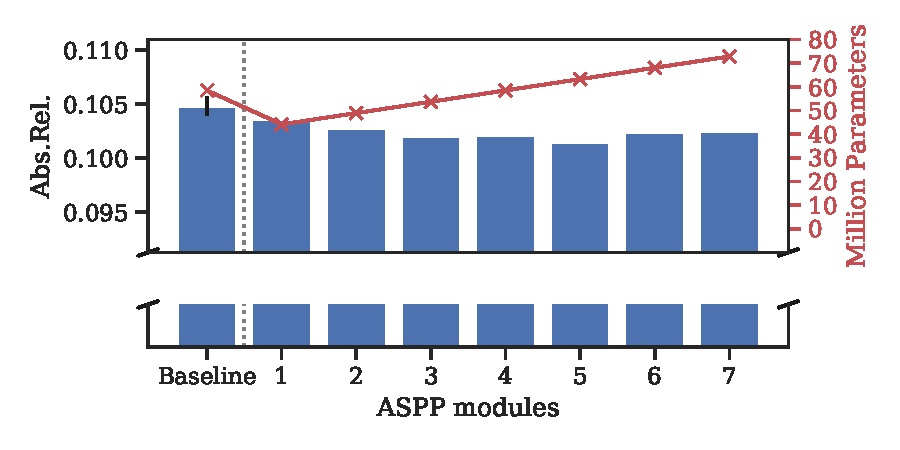
\includegraphics[width=1.0\linewidth]{images/figures/experiment2_AbsRel.pdf}
    \end{center}
   \caption{Absolute relative error of architectures with a different number of ASPP modules. The error bar indicates the standard deviation of the abs. rel. error of our baseline implementation. Additionally, the number of network parameters is plotted for each architecture.}
\label{fig:long}
\end{figure}
Since the network with four standard convolutions in parallel inside the ASPP performed best, we investigated the impact of the number of these convolutional layers.
\figurename~\ref{fig:long} shows the abs. rel. error for models with increasing number of standard convolutions in the ASPP, along with the number of parameters.
One can see, that adding one convolutional layer increases the parameter count by about 4 million, while slightly improving error metrics on the evaluation. This trend starts to decline after more than 5 convolutions are added. 

\subsection{Atrous Convolutions in the Encoder}\label{section:experiments:atrous-encoder}
In the previous, we saw that adding an ASPP module at the end of the encoder, which was successfully done in the DeepLab Architecture for segmantic segmentation~\cite{chen2018deeplab, chen2018encoder}, impaired depth estimation when atrous rates larger than 1 were used.
Therefore, we asked whether depth prediction would benefit from employing atrous convolutions with different rates between or within earlier layers of the encoder (see supplementary \figurename~\ref{fig:appendix:aspp-encoder} and \figurename~\ref{fig:appendix:resnet-atrous}). 

In the first experiment we placed the entire ASPP module between ResNet block 1 and 2 to obtain feature responses at different spatial scales at an earlier stage of the encoder.
At this stage the image has only been resized to $64\times32$ corresponding to an output stride of 8. As an initial exploration, we compared a model with only standard convolutions  (rates [1,1,1,1]) against a model with atrous rates [1,6,12,18] (the default values in DeepLab~\cite{chen2018deeplab}). The model with only standard convolutions performed better than the one with atrous convolutions (see supplementary Table~\ref{table:appendix:aspp-encoder}). Thus, we did not further explore this direction and focused on placing the ASPP after the encoder.

In the second experiment we employed atrous convolutions within the ResNet blocks themselves. Again, all other ASPP rates larger than 1 harmed the depth prediction performance as can be seen by an increase in the error metrics compared to the baseline (see supplementary \tablename~\ref{table:appendix:atrous-encoder}).

\subsection{Evaluation on Virtual KITTI}\label{section:vkitti}
Our goal is to evaluate whether atrous convolutions help with monocular depth estimation, especially if they improve the sharpness at object boundaries. Since the KITTI Stereo 2015 ground truth data is rather sparse, it might not contain data points at exactly those most relevant positions at object boundaries. Synthetic data, on the other hand, provides exact ground truth depth at every single pixel. For this reason, we evaluated the models presented in the previous sections on the Virtual KITTI (VKITTI) dataset~\cite{Gaidon:Virtual:CVPR2016}. Because it only provides monocular images, we could not use it for training but only for evaluation. VKITTI contains clones of five sequences from the original KITTI Vision Benchmark Suite~\cite{geiger2012we} in different weather conditions. To keep these weather conditions identical to the training set, we only chose those sequences that are exact clones of the original sequences, yielding 2126 images in total.
\begin{figure}
    \centering
    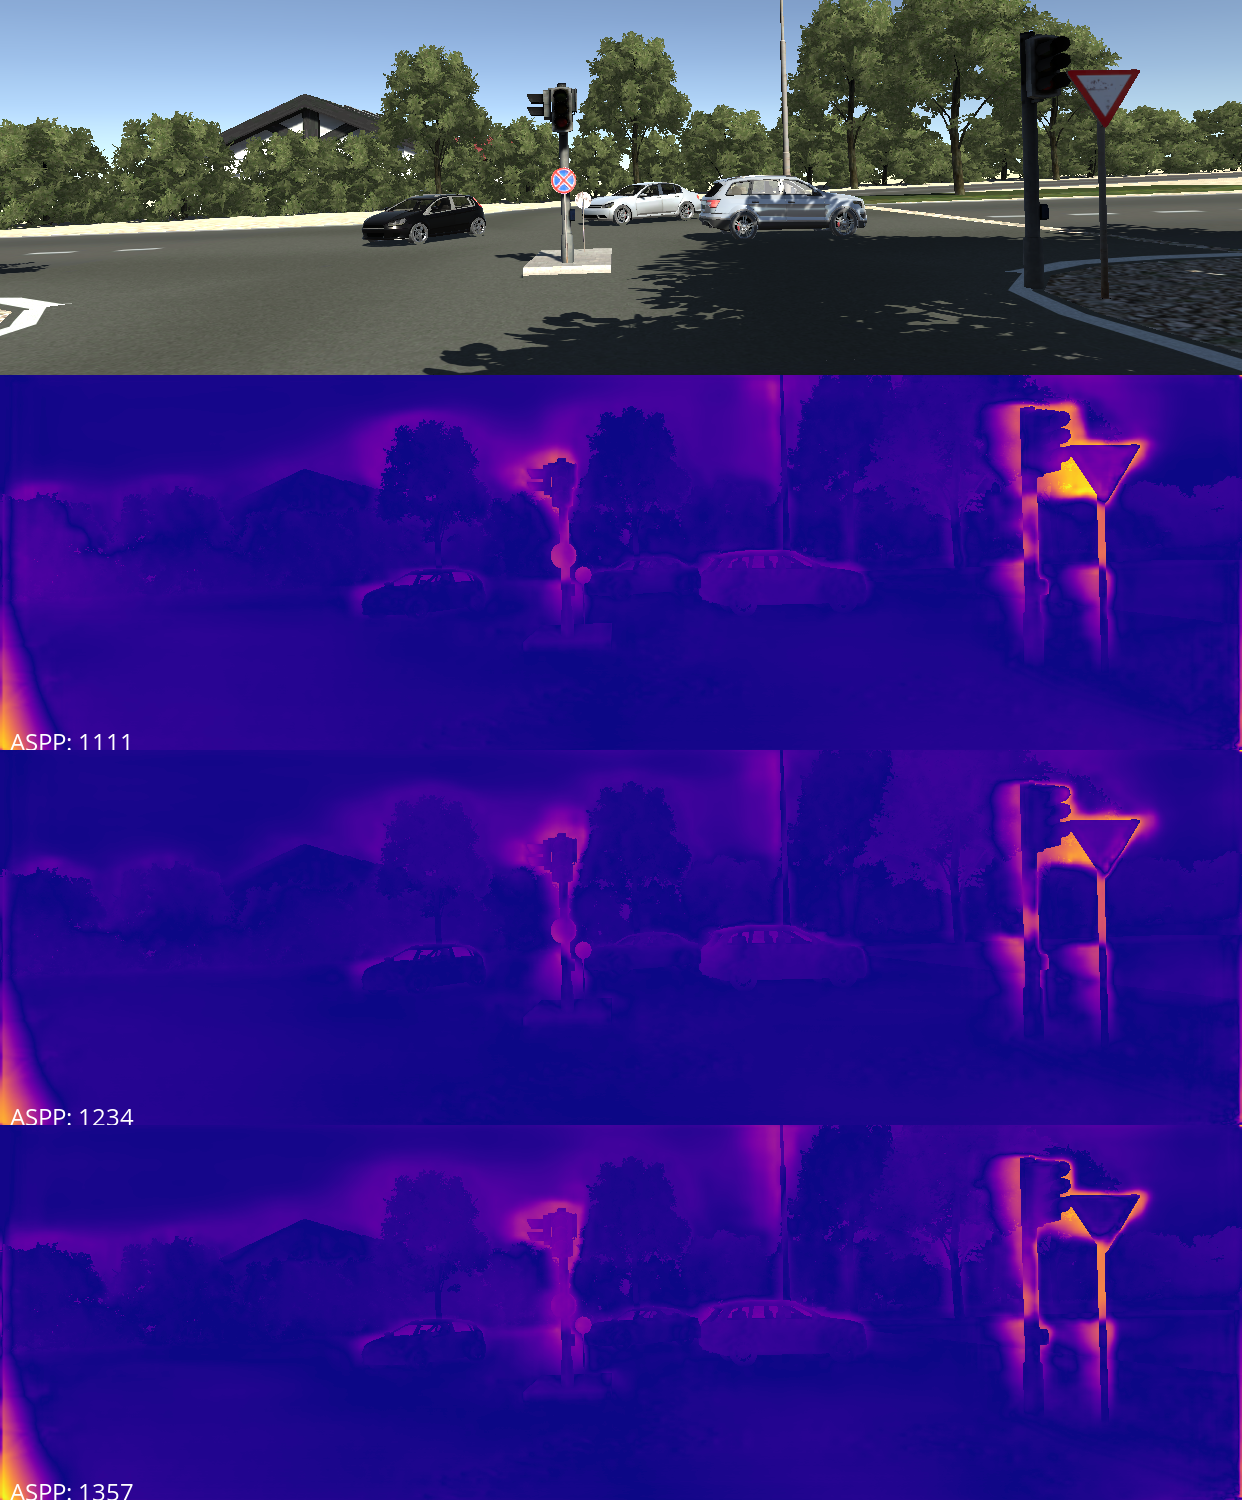
\includegraphics[width=0.85\linewidth]{images/visual_comparisons/aspp-rates-vkitti/concat_383.png}
    \caption{Disparity error maps (absolute difference between predicted and ground truth disparity) on VKITTI. Atrous rates from top to bottom: [1,1,1,1], [1,2,3,4], [1,3,5,7]. Error maps for additional images are available in the supplementary \figurename~\ref{fig:appendix:vkitti}.}
    \label{fig:vkitti}
\end{figure}

% Keep table here due to placement issues
\begin{table*}[h!]
   \centering
   \small
   \setlength{\tabcolsep}{4pt}
   \begin{tabular}{lrllrrrrrrrrr}
\toprule
 Model & Output-stride &     ASPP &  Abs.Rel. &  Sq.Rel. &   RMSE &  Log RMSE &     a1 &     a2 &     a3 &      Params (M) & $\Delta$ Abs. Rel. (\%)\\
\midrule
       Godard & 64  &      - &    0.0970 &   0.8960 &  5.093 &     0.176 &  0.962 &  0.962 &  0.986 &         58.4 & -- \\
       Godard & 16 & - & 0.0955 & 0.8752 &      4.937 &      0.174 &     0.881 &      0.961 &    0.984 & 58.4 & 2.57 \\
            Ours (A) & 16 &  1-1-1-1 &    \textbf{0.0927} &   \textbf{0.8132} &  \textbf{4.865} &     \textbf{0.168} &  \textbf{0.888} &  \textbf{0.967} &  \textbf{0.987} &         58.4 & \textbf{4.43} \\
            Ours (B) & 16 &   1 &    0.0944 &   0.8446 &  5.011 &     0.174 &  0.884 &  0.963 &  0.986 &         \textbf{44.1} & 2.68 \\ \bottomrule \end{tabular}
   \caption{Final model comparison.
   Each model was pretrained on the Cityscapes dataset and evaluated on KITTI Stereo 2015 after applying postprocessing as in \cite{Godard_2017_CVPR}. 
   The last column measures the relative difference of the abs. rel. error to the original model from Godard~\etal~\cite{Godard_2017_CVPR}.}
   \label{table:best-models}
\end{table*}
\figurename~\ref{fig:vkitti} shows disparity error maps for the models with different atrous rates from Section \ref{section:aspp-rates} at output stride 32. As on KITTI, all models have problems predicting disparity accurately at the object boundaries. Upon visual inspection of the disparity maps, there is no apparent difference between the models with different atrous rates. Numerical evaluation did also not provide any clear conclusions w.r.t. the effectiveness of atrous convolutions.

\subsection{Improvement over Baseline}
% Best models table

Summarizing the previous experiments, \tablename~\ref{table:best-models} shows our most interesting models in comparison to the baseline model of Godard \etal~\cite{Godard_2017_CVPR} and illustrates some trade-offs when making architectural decisions.
\begin{figure}
    \centering
    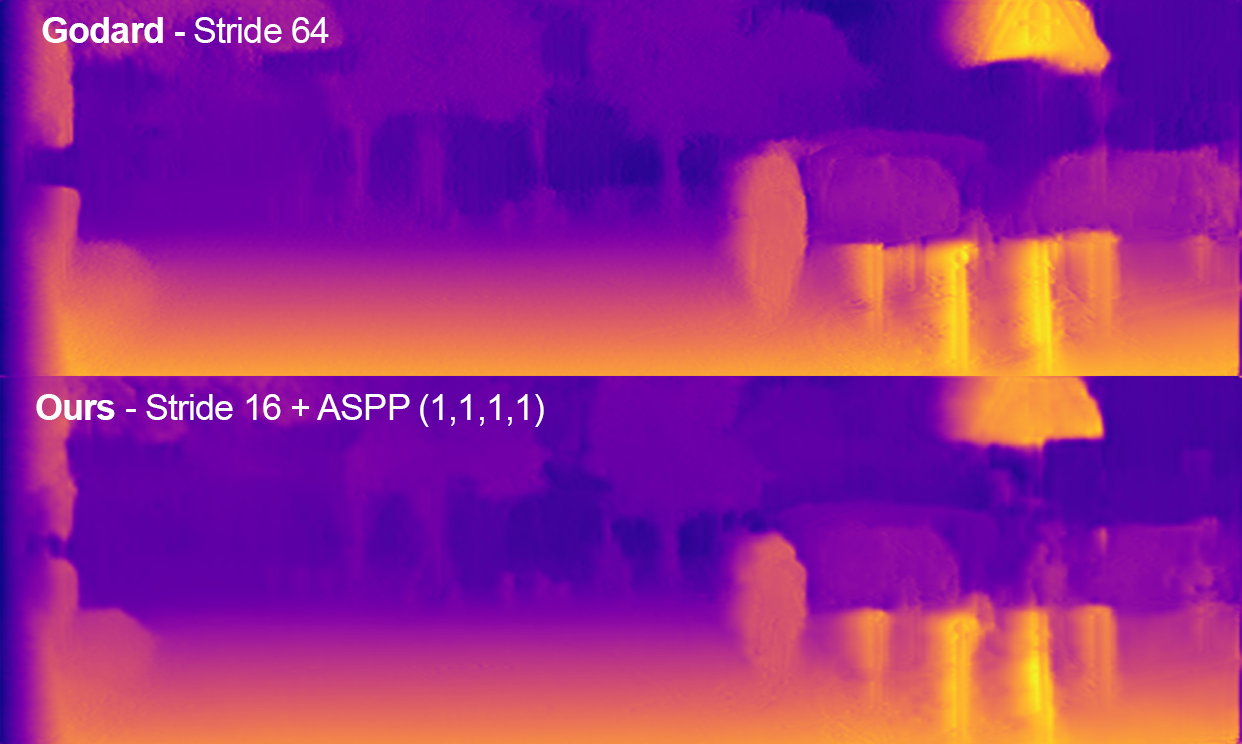
\includegraphics[width=0.8\linewidth]{images/disparities/final_godard_comparison.png}
    \caption{Disparity map comparison of our best model to the baseline~\cite{Godard_2017_CVPR}. There are no obvious visual differences.}
    \label{fig:final-comparison}
\end{figure}
Our best performing model, using an output stride of 16 and four ASPP modules with an atrous rate of 1, achieves an improvement of 4.43\% in the abs. rel. error over the baseline model while having the same number of parameters (model A). There is, however, no clear improvement in terms of visual inspection of the disparity maps (see \figurename~\ref{fig:final-comparison}.
When we further degenerate the ASPP block to only use the very first $1 \times 1$ module, we can reduce the number of parameters by 24.5\%, while still achieving an improvement of 2.68\% over Godard \etal~\cite{Godard_2017_CVPR} (model B).



%%%%%%%%% CONCLUSION
\section{Conclusion}
We have presented the idea and results for the incorporation of atrous convolutions into Godard \etal's~\cite{Godard_2017_CVPR} unsupervised monocular depth estimation framework using left-right consistency.
Experiments with atrous convolutions were mainly conducted using the Atrous Spatial Pyramid Pooling block, inserted between the encoder and decoder, which was already successful in the task of image segmentation~\cite{chen2018deeplab}.
We conclude, that atrous convolutions within the presented experiments do not improve monocular depth estimation. Furthermore, the use of atrous convolutions enforces a higher output stride which consequently harms runtime and memory consumption.

In the event of these experiments we additionally found out, that in Godard \etal's~\cite{Godard_2017_CVPR} architecture, it is possible to reduce the number of channels between the encoder and decoder. This can decrease the number of network parameters and improve runtime, without losing predictive power.

Our experiments focused on architectural design instead of hyperparameter tuning. Finding the optimal set of hyperparameters for models with atrous convolutions might lead to different results. Future work should investigate why atrous convolutions work so well in semantic segmentation, but cannot be applied straightforwardly to continuous depth estimation. In semantic segmentation, there is a clear distinction between object classes, while regression problems face the harder problem of predicting a continuous signal. Recent work suggests that atrous convolutions help if depth estimation is treated as a classification problem with discrete depths \cite{Fu2018}. Alternatively, semantic features could be leveraged to improve depth estimation performance \cite{Jiao2018}, in which case atrous convolutions might be helpful.


{\small
\bibliographystyle{ieee}
\bibliography{bibliography}
}

\clearpage
%%%%%%%%% APPENDICES
\appendix
\onecolumn
\begin{center}
\textbf{\Large Unsupervised Monocular Depth Estimation Using Atrous Convolutions}
\textbf{\large Supplementary Material}
\end{center}

\setcounter{figure}{0}
\renewcommand\thefigure{\thesection.\arabic{figure}}
\setcounter{table}{0}
\renewcommand{\thetable}{\thesection.\arabic{table}}

\section{Atrous Convolutions in the Encoder}\label{appendix:atrous-encoder}
\setcounter{figure}{0}  
    
    \begin{figure}[ht]
    \centering
    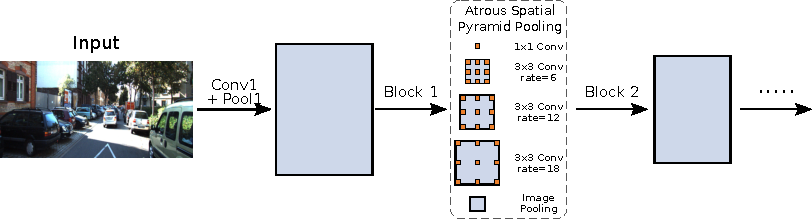
\includegraphics[width=0.8\textwidth]{images/architecture/aspp-in-encoder.pdf}
    \caption{ASPP after the first ResNet block.}
    \label{fig:appendix:aspp-encoder}
    \end{figure}
    \begin{figure}[ht]
    \centering
    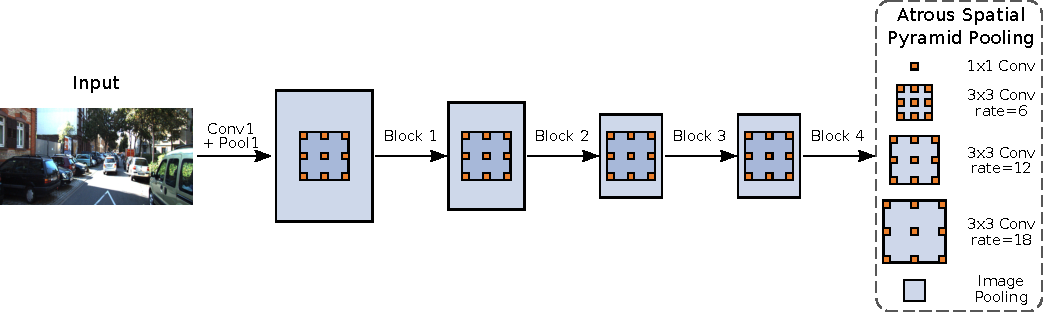
\includegraphics[width=0.8\textwidth]{images/architecture/encoder-with-atrous-rates.pdf}
    \caption{Atrous convolutions inside the ResNet blocks.}
    \label{fig:appendix:resnet-atrous}
    \end{figure}
    
     
\section{Reconstruction error plots}
\setcounter{figure}{0}    
% the \\ insures the section title is centered below the phrase: AppendixA

\begin{figure}[h!]
\centering
\begin{subfigure}[c]{0.24\textwidth}
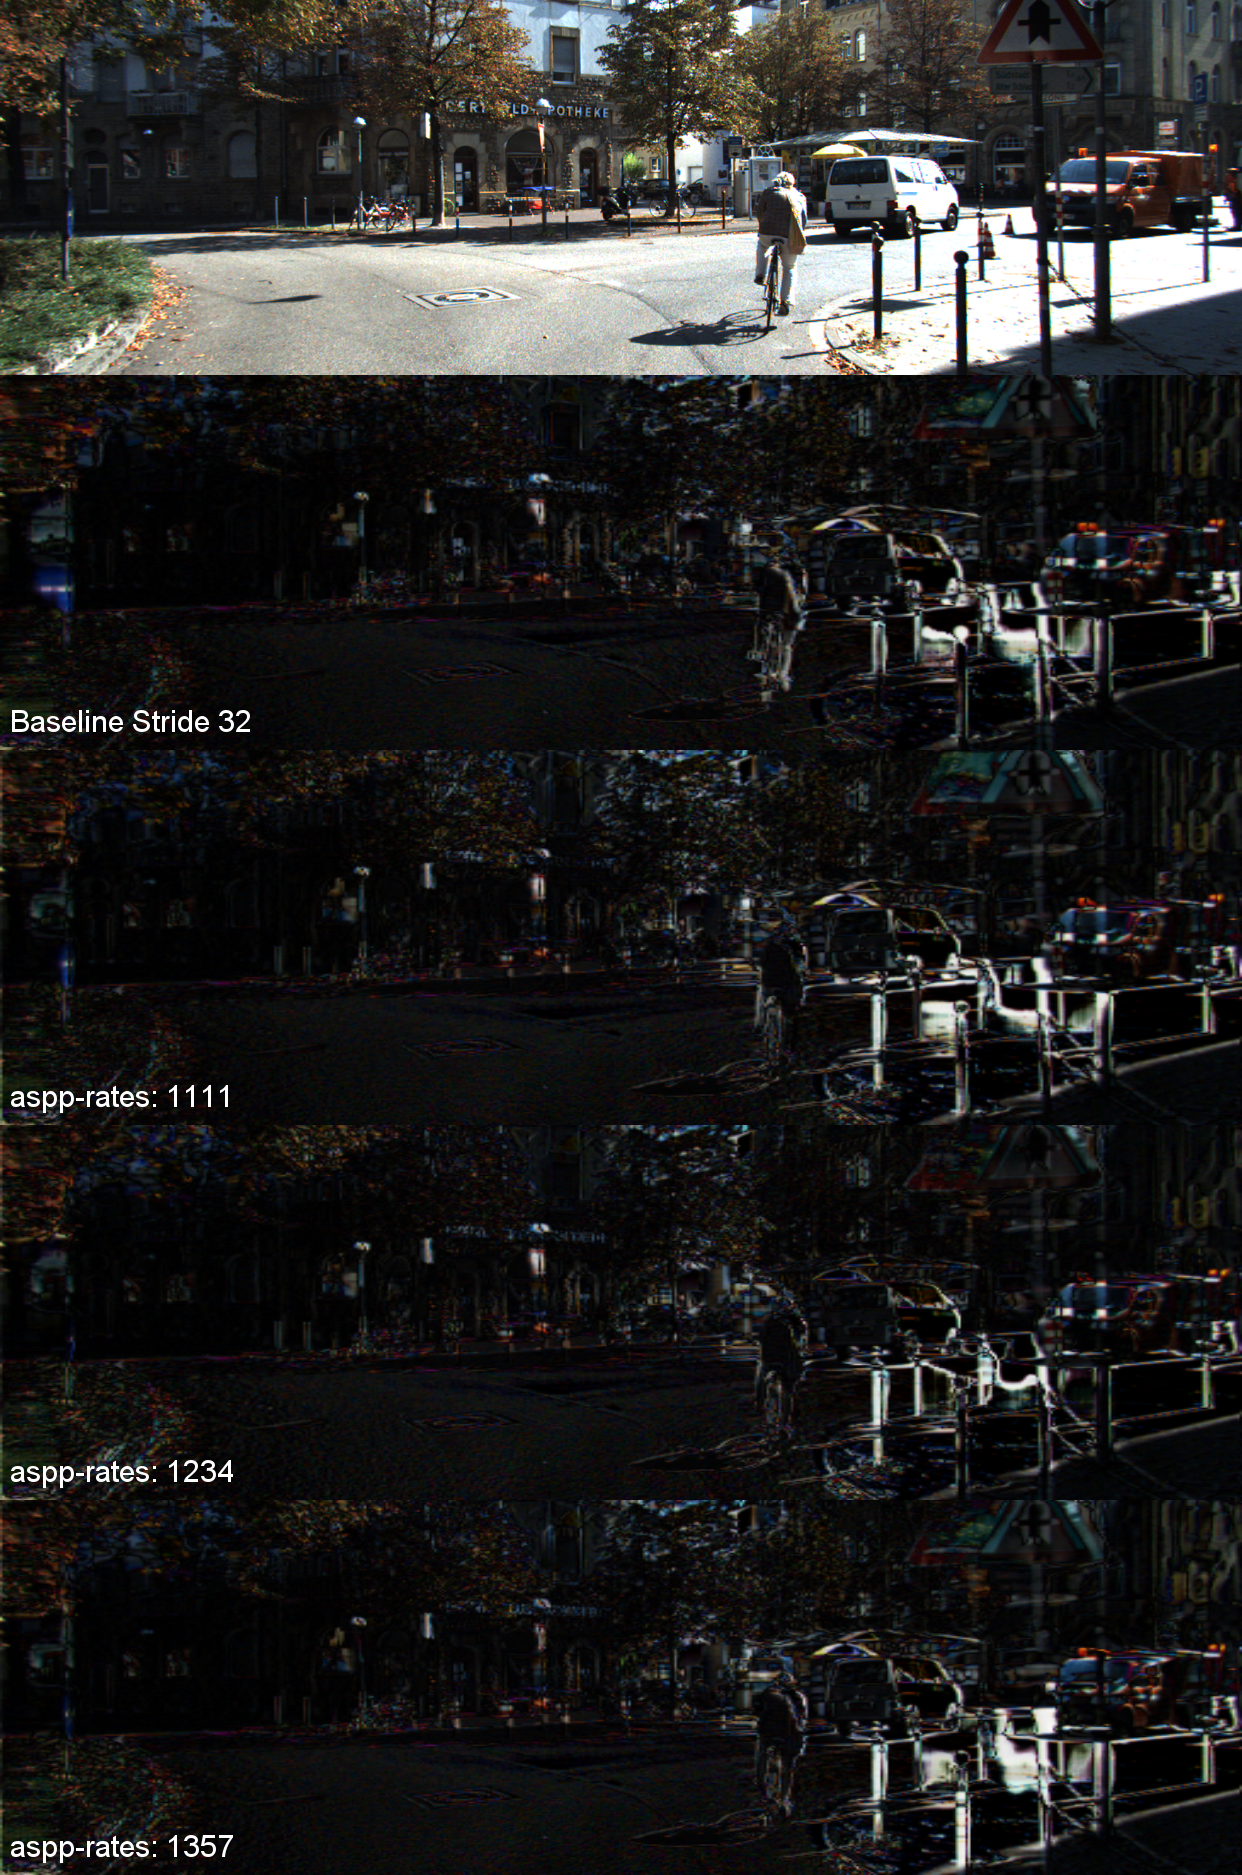
\includegraphics[width=\textwidth]{images/visual_comparisons/reconstruction_error/concat_003.png}
\end{subfigure}
\begin{subfigure}[c]{0.24\textwidth}
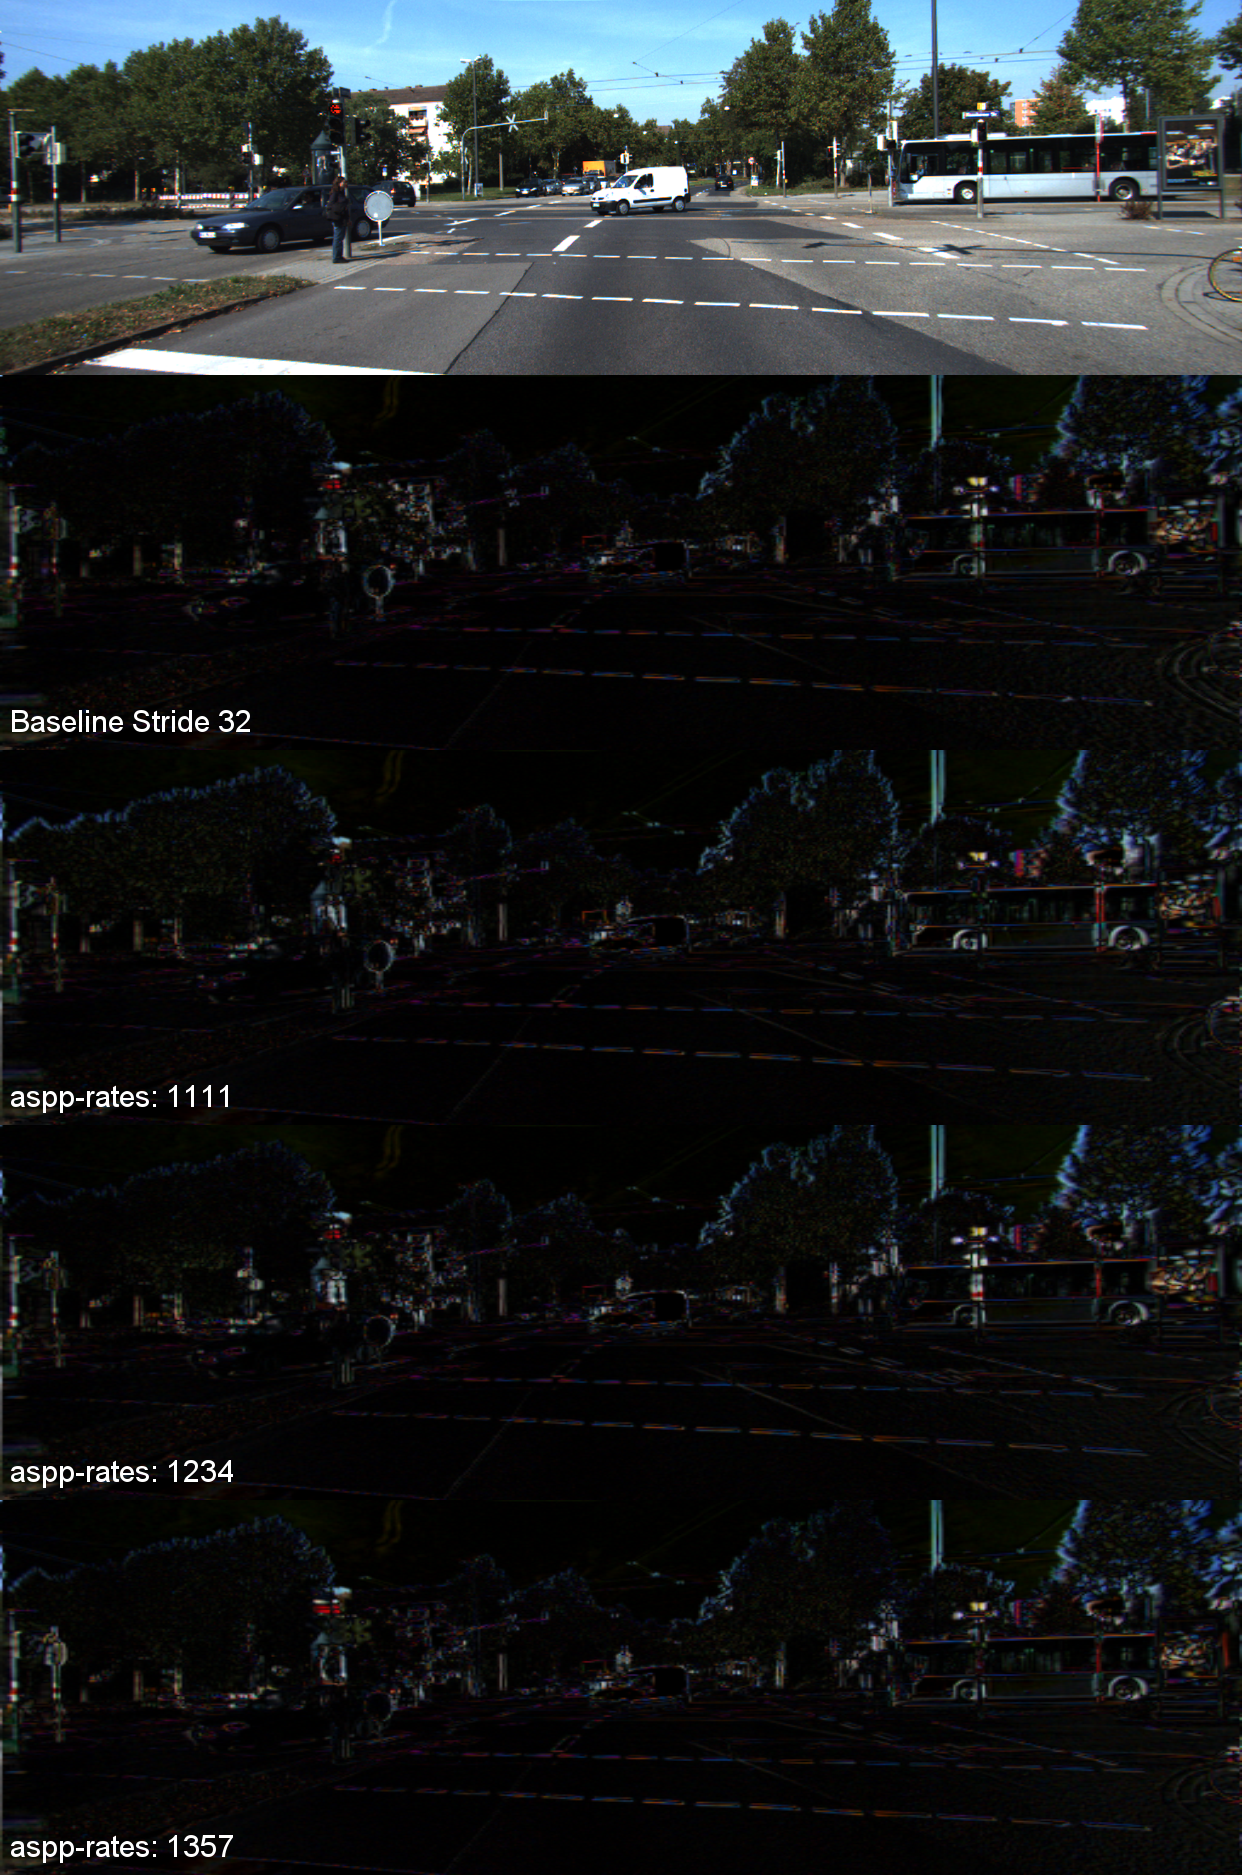
\includegraphics[width=\textwidth]{images/visual_comparisons/reconstruction_error/concat_015.png}
\end{subfigure}
\begin{subfigure}[c]{0.24\textwidth}
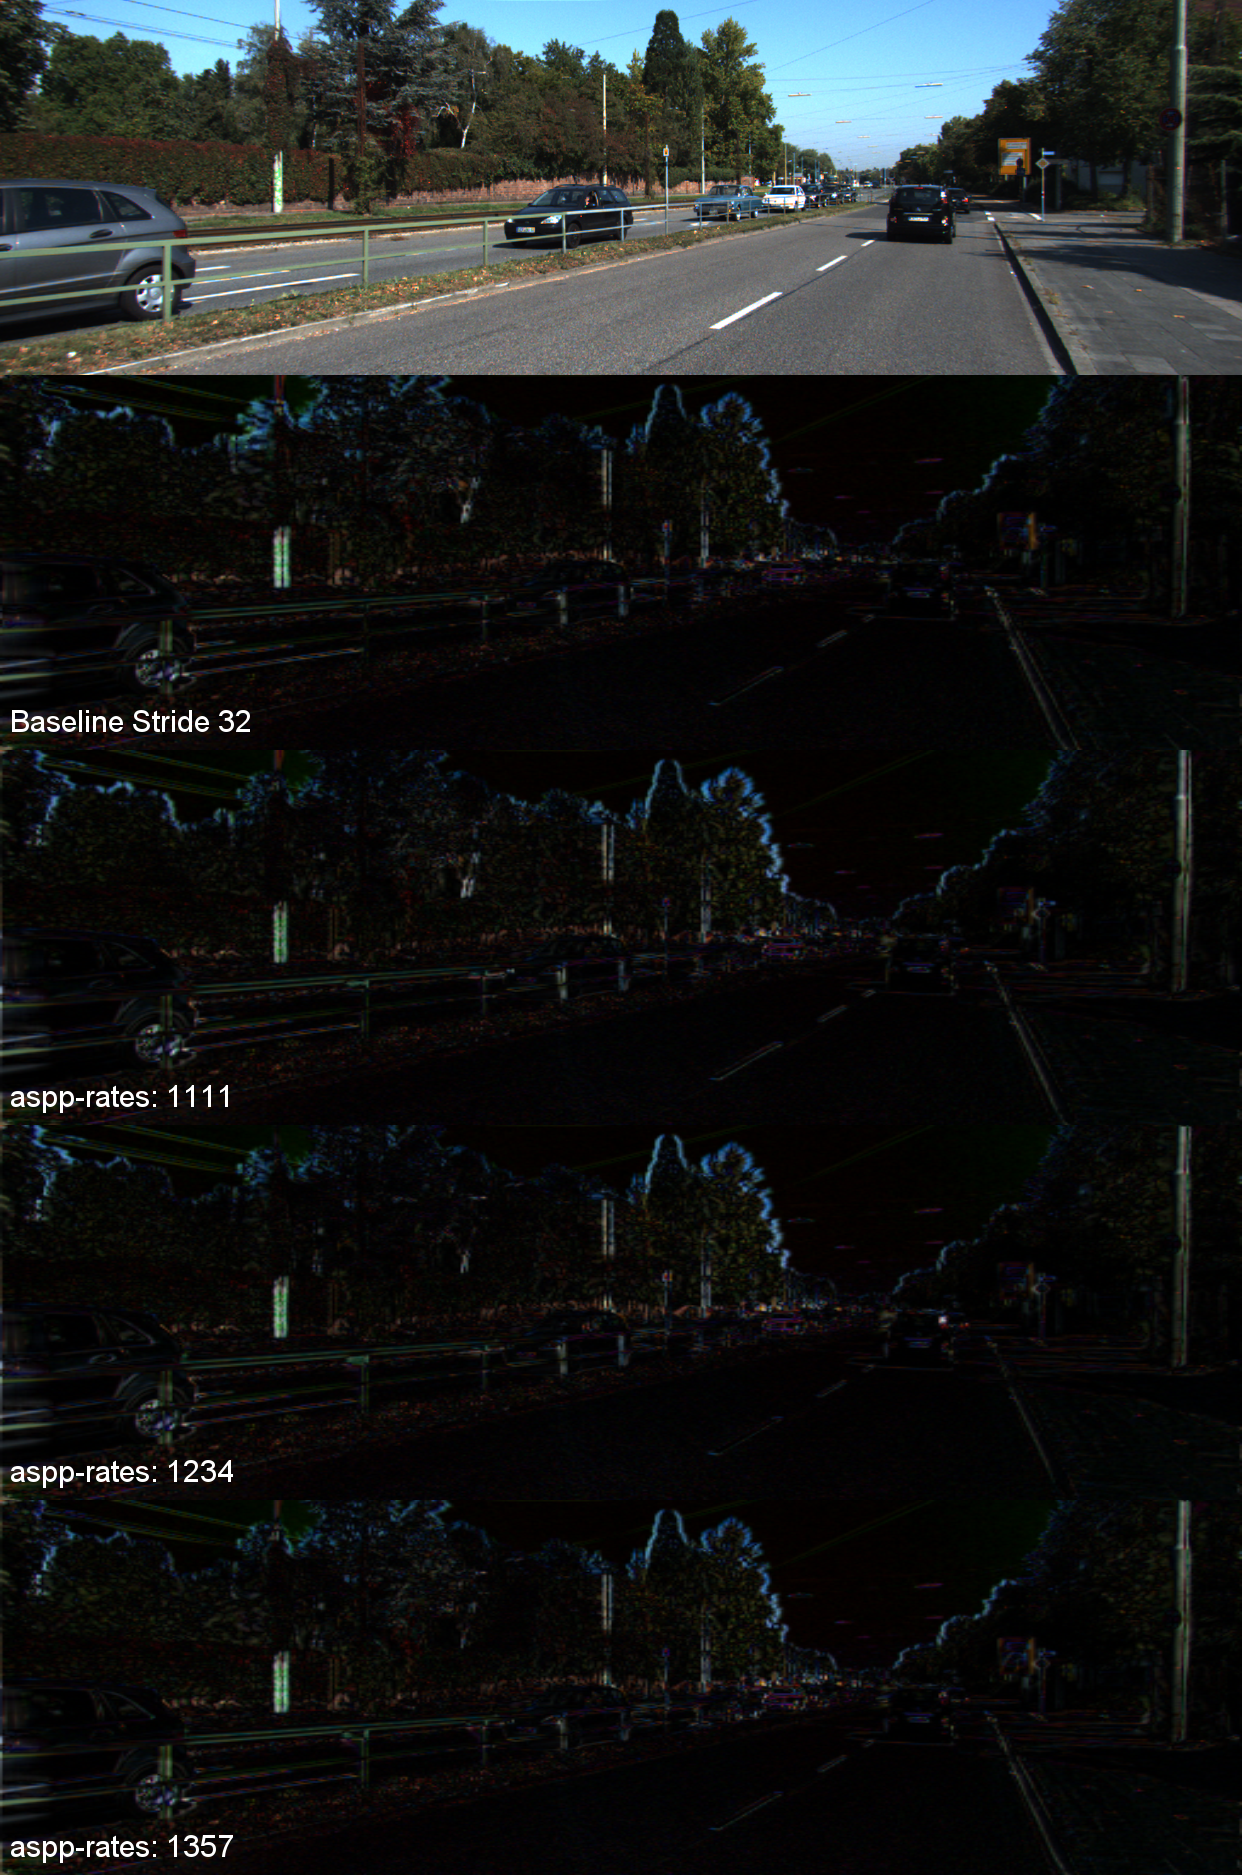
\includegraphics[width=\textwidth]{images/visual_comparisons/reconstruction_error/concat_024.png}
\end{subfigure}
\begin{subfigure}[c]{0.24\textwidth}
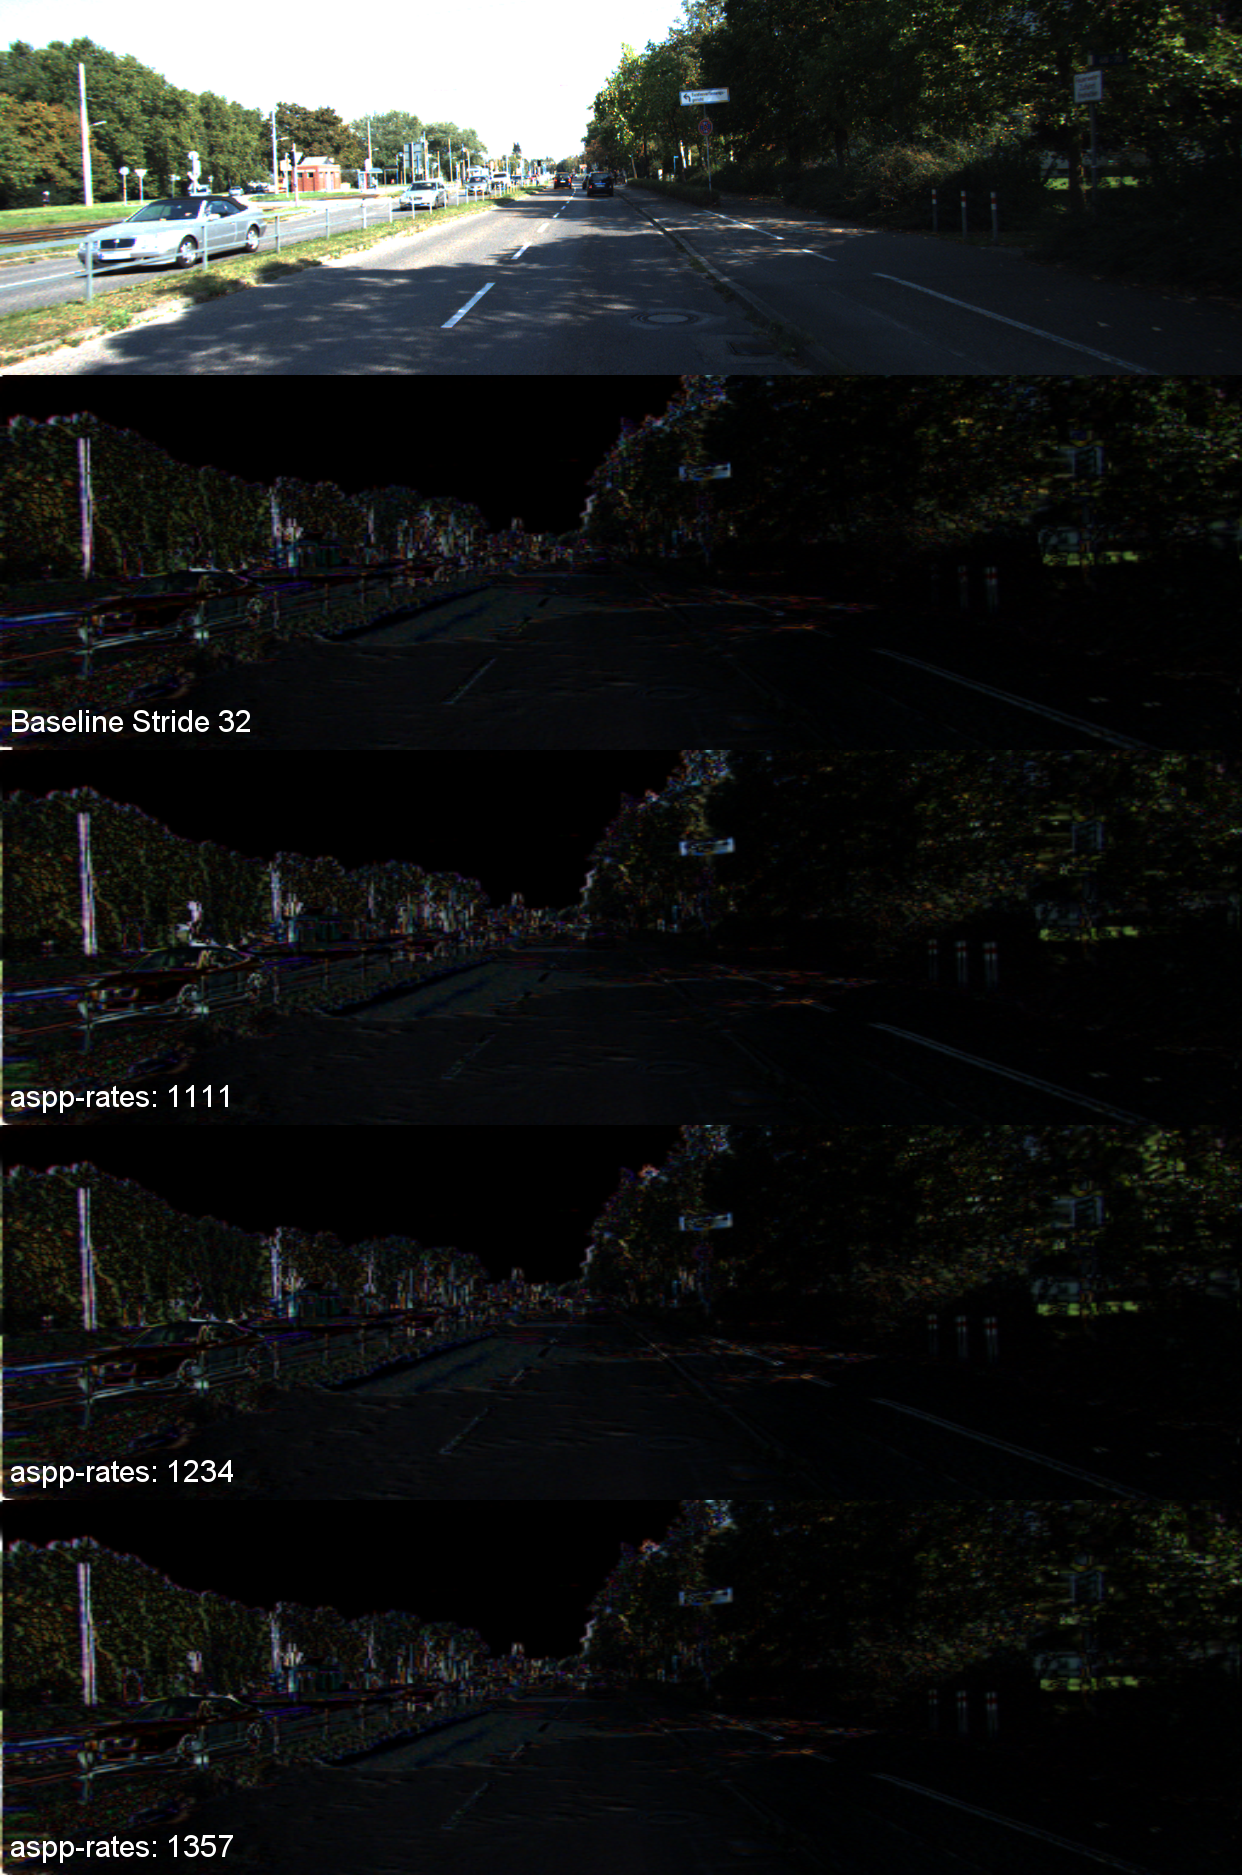
\includegraphics[width=\textwidth]{images/visual_comparisons/reconstruction_error/concat_029.png}
\end{subfigure}
\caption{Reconstruction error for the experiment in Section \ref{section:aspp-rates} in which the impact of different atrous rates ([1,1,1,1], [1,2,3,4], [1,3,5,7]) was compared to the baseline.}
\label{appendix:reconstruction-error}
\end{figure}

\section{VKITTI Error Maps}
\begin{figure}[h!]
\centering
\begin{subfigure}[c]{0.24\textwidth}
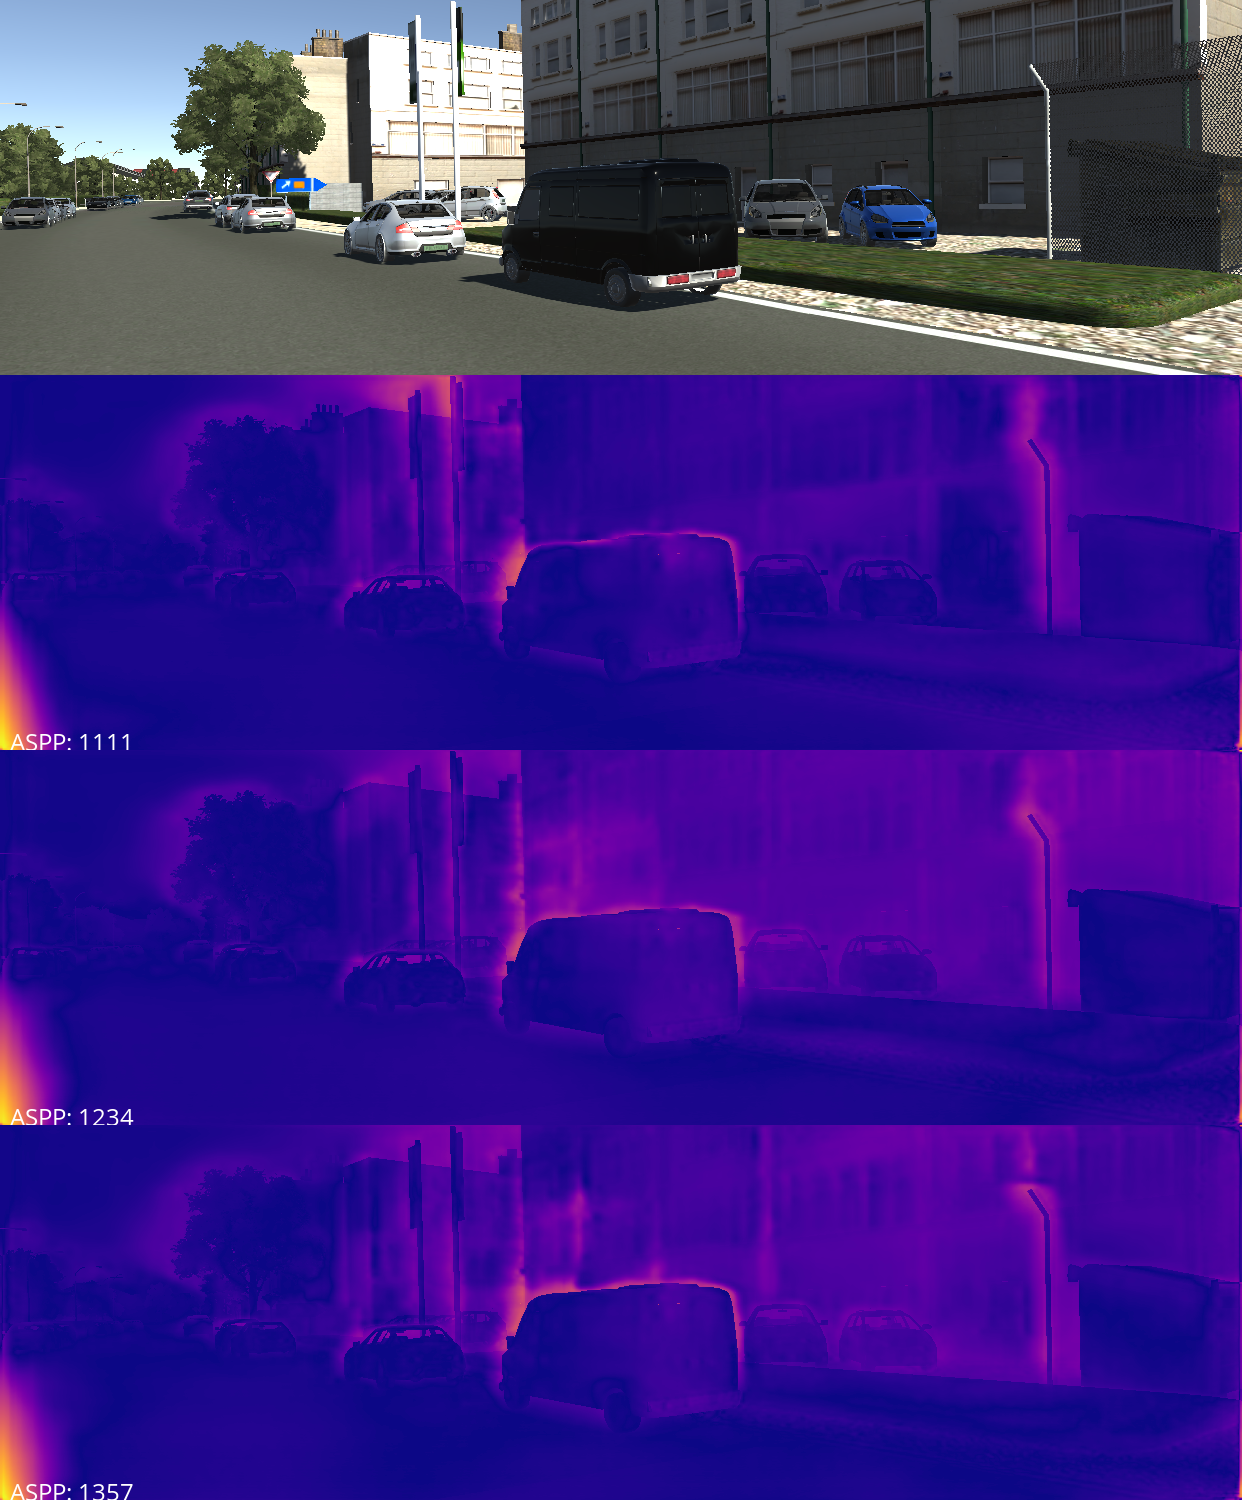
\includegraphics[width=\textwidth]{images/visual_comparisons/aspp-rates-vkitti/concat_221.png}
\end{subfigure}
\begin{subfigure}[c]{0.24\textwidth}
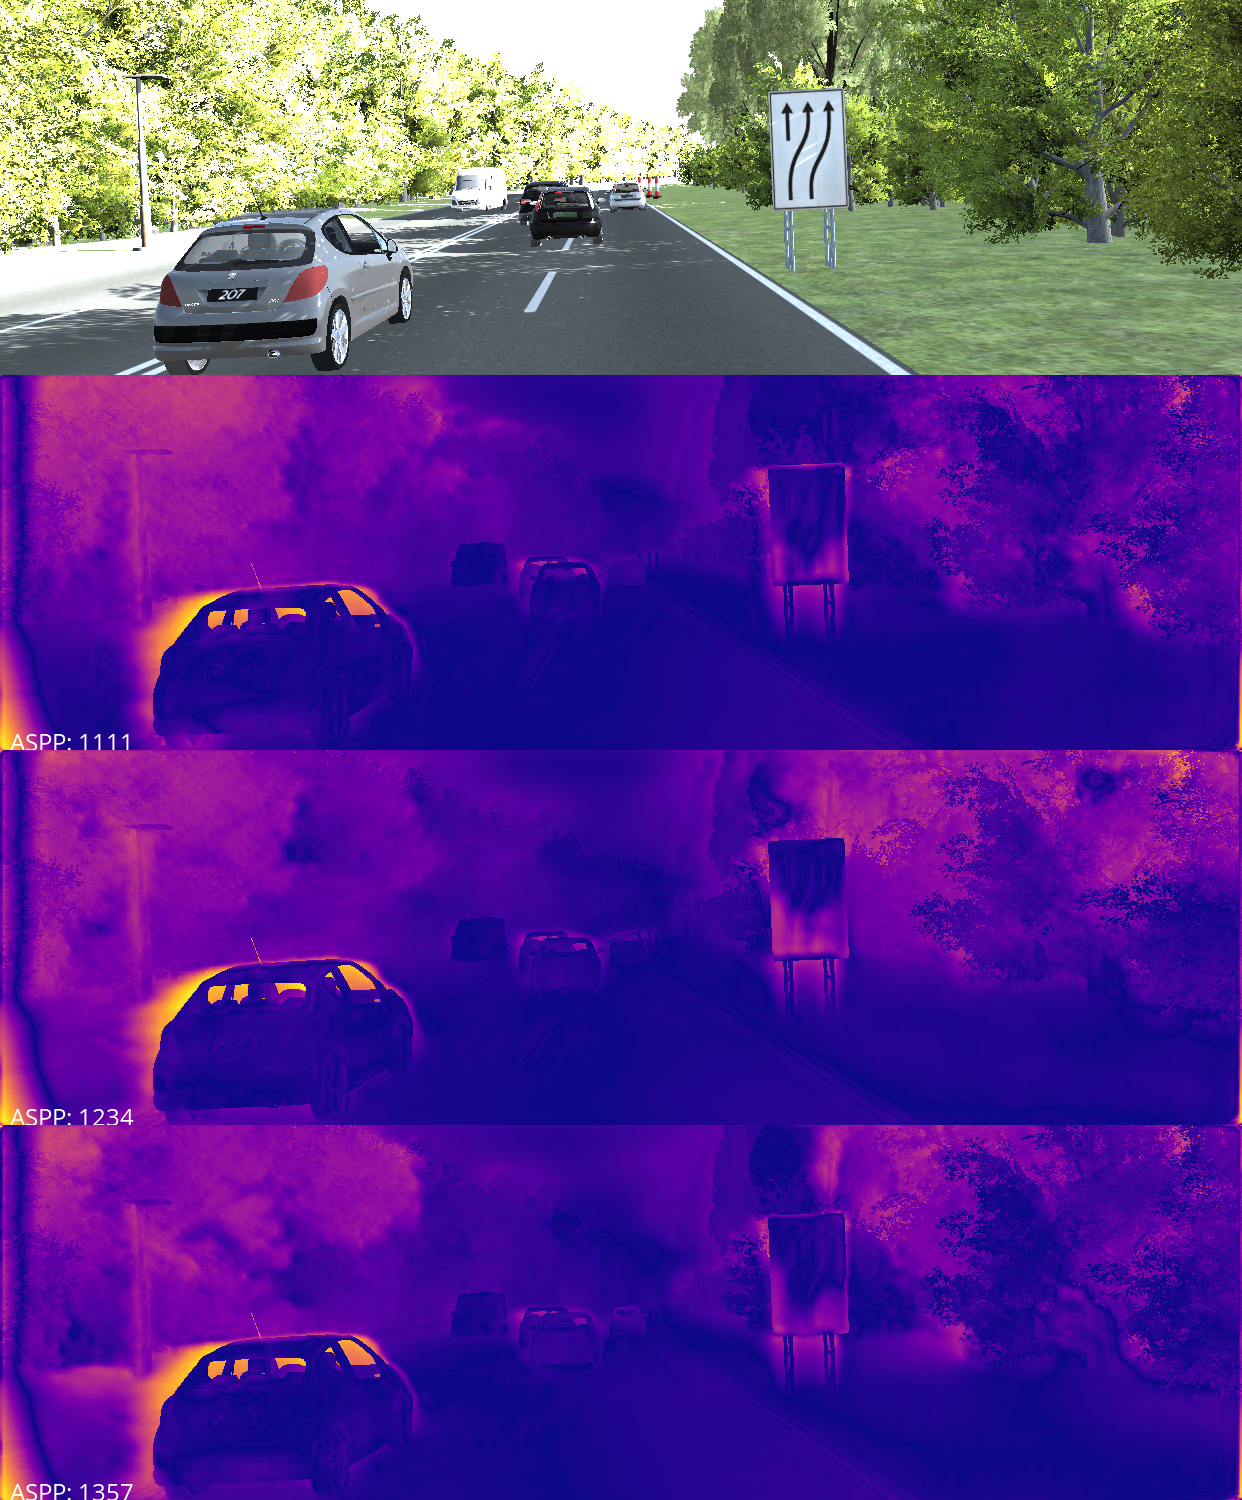
\includegraphics[width=\textwidth]{images/visual_comparisons/aspp-rates-vkitti/concat_1226.png}
\end{subfigure}
\begin{subfigure}[c]{0.24\textwidth}
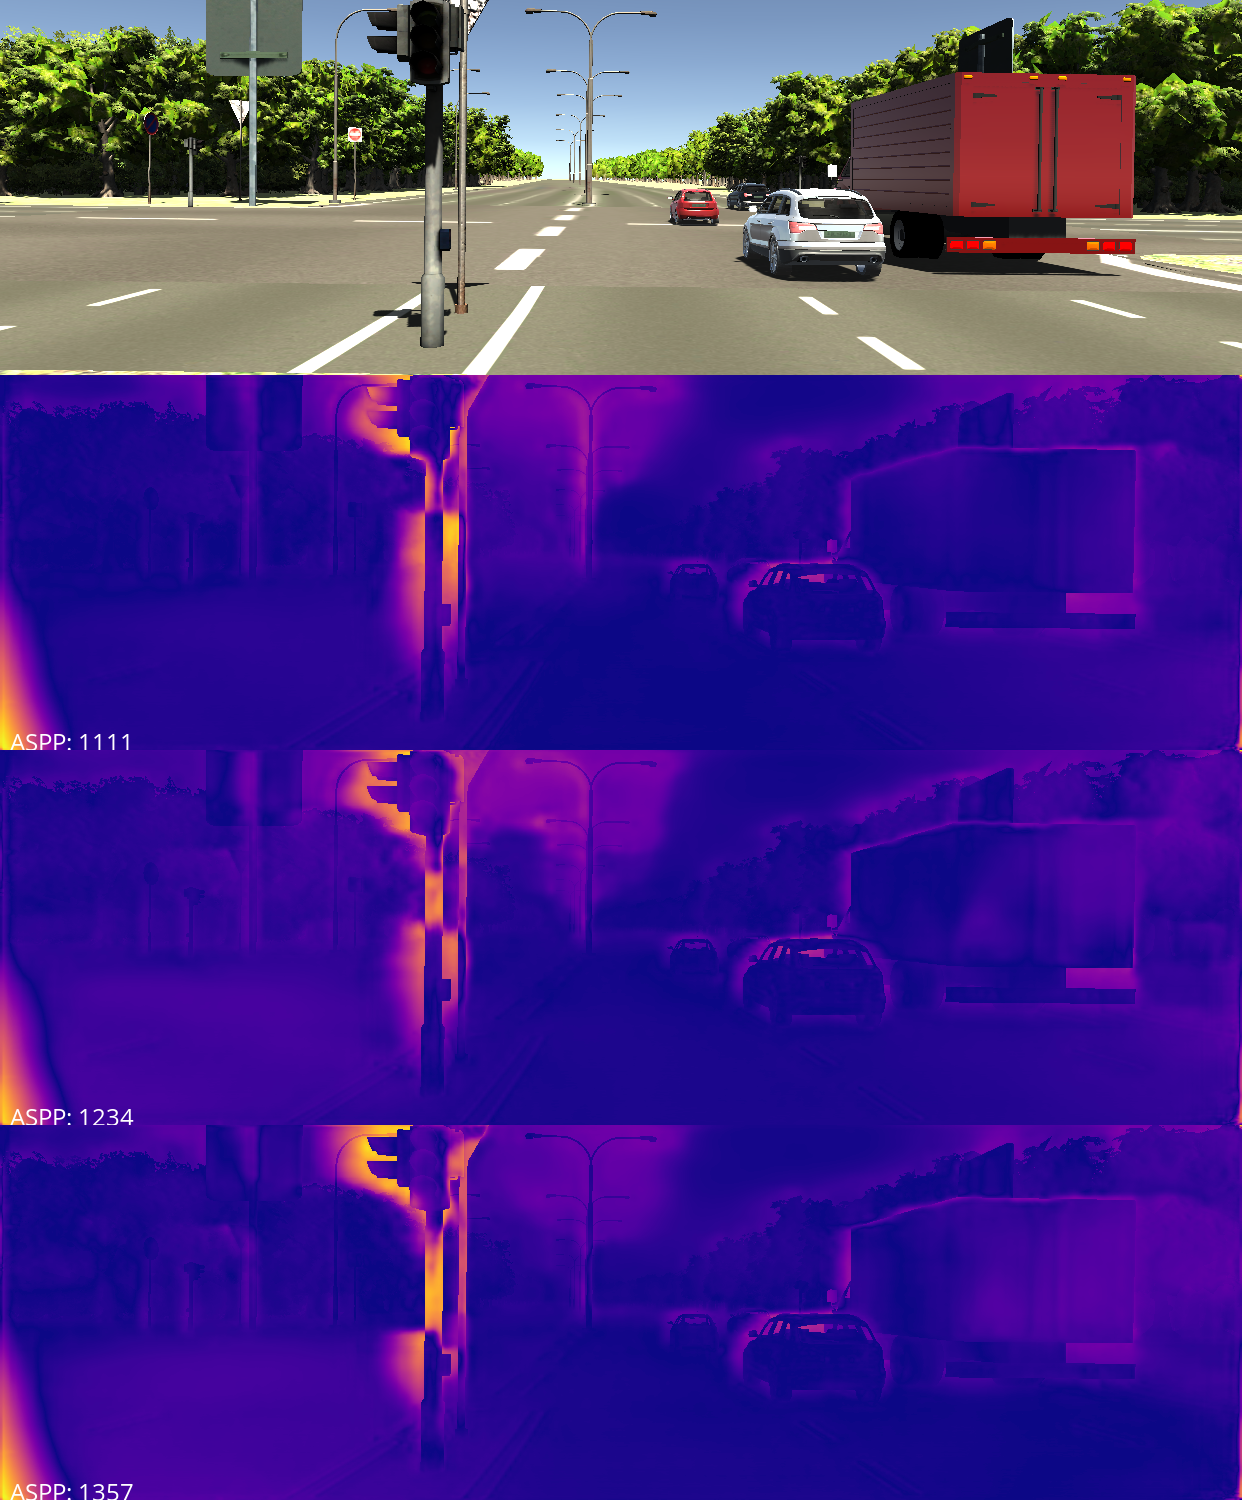
\includegraphics[width=\textwidth]{images/visual_comparisons/aspp-rates-vkitti/concat_763.png}
\end{subfigure}
\begin{subfigure}[c]{0.24\textwidth}
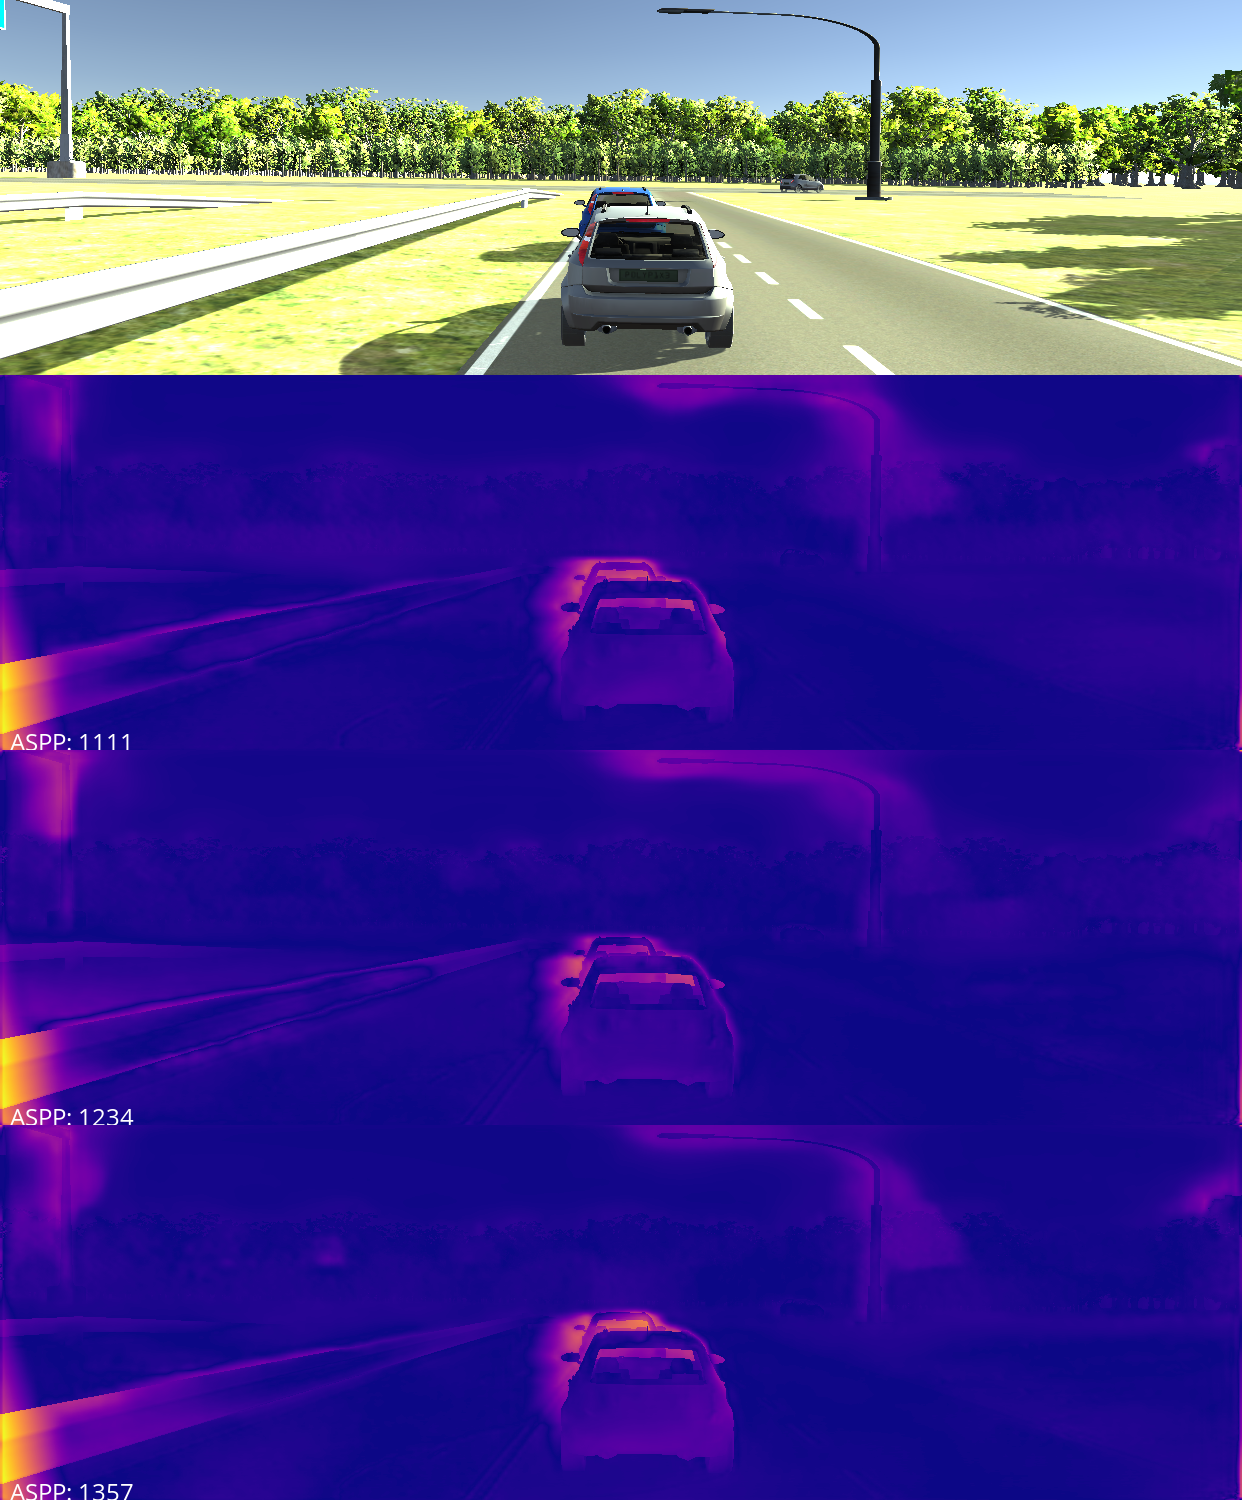
\includegraphics[width=\textwidth]{images/visual_comparisons/aspp-rates-vkitti/concat_2083.png}
\end{subfigure}
\caption{Disparity error maps on VKITTI (cf. Section \ref{section:vkitti}), in which the impact of different atrous rates ([1,1,1,1], [1,2,3,4], [1,3,5,7]) are compared.}
\label{fig:appendix:vkitti}
\end{figure}


\section{Full Experimental Results}\label{appendix:full-results}
\setcounter{figure}{0}    
% the \\ insures the section title is centered below the phrase: Appendix B


\begin{table}[ht]
    \centering
    \begin{tabular}{lllrrrrrrrrr}
    \toprule
     Output-stride & Abs.Rel. &  Sq.Rel. &   RMSE &  Log RMSE &     $\delta < 1.25^1$ &     $\delta < 1.25^2$ &     $\delta < 1.25^3$ &      Params (M) \\
    \midrule 
           8   &   0.1068  &  1.0408  &  5.533  &  0.197  &  0.859  &  0.946  &  0.979 & 58.4\\
           16  &   0.1041  &  1.0097  &  5.362  &  0.191  &  0.865  &  0.951  &  0.981 & 58.4\\
           32  &   0.1048  &  1.0353  &  5.458  &  0.191  &  0.866  &  0.949  &  0.980 & 58.4\\
           64  &   0.1120  &  1.2025  &  5.716  &  0.201  &  0.854  &  0.948  &  0.981 & 58.4\\
    \bottomrule
    \end{tabular}
    \caption{Comparison of output stride 8, 16, 32 and 64.}
\end{table}


\begin{table}[ht]
    \centering
    \begin{tabular}{lllrrrrrrrrr}
    \toprule
     Output-stride & ASPP &  Abs.Rel. &  Sq.Rel. &   RMSE &  Log RMSE &     $\delta < 1.25^1$ &     $\delta < 1.25^2$ &     $\delta < 1.25^3$ &      Params (M) \\
    \midrule 
           16  &  1-1-1-1 &   0.1007  &  0.9439  &  5.322  &  0.186  &  0.871  &  0.956  &  0.983 & 58.4\\
           16  &  1-2-3-4 &   0.1038  &  0.9571  &  5.351  &  0.187  &  0.867  &  0.956  &  0.980 & 58.4\\
           16  &  1-3-5-7 &   0.1058  &  0.9803  &  5.472  &  0.192  &  0.864  &  0.95-  &  0.981 & 58.4 \\
           \addlinespace
           32  &  1-1-1-1 &   0.1021  &  0.9561  &  5.300  &  0.185  &  0.870  &  0.956  &  0.984 & 58.4 \\
           32  &  1-2-3-4 &   0.1037  &  1.0007  &  5.446  &  0.190  &  0.869  &  0.954  &  0.983 & 58.4 \\
           32  &  1-3-5-7 &   0.1055  &  1.0374  &  5.421  &  0.191  &  0.866  &  0.951  &  0.982 & 58.4 \\
    \bottomrule
    \end{tabular}
    \caption{Experiment on the influence of increasing atrous rates in the ASPP block for output stride 16 and 32. For both output strides, increasing the atrous rates has increased the depth estimation error on all metrics.}
\end{table}


\begin{table}[ht]
    \centering
    \setlength{\tabcolsep}{4pt}
    \begin{tabular}{lllrrrrrrrrr}
    \toprule
     Output-stride & ASPP &  Abs.Rel. &  Sq.Rel. &   RMSE &  Log RMSE &     $\delta < 1.25^1$ &     $\delta < 1.25^2$ &     $\delta < 1.25^3$ &      Params (M) \\
    \midrule 
           32  &  1             &   0.1036  &  1.0123  &  5.403  &  0.187  &  0.867  &  0.955  &  0.984 & 44.1 \\
           32  &  1-1           &   0.1027  &  1.0260  &  5.373  &  0.188  &  0.872  &  0.955  &  0.983 & 48.9 \\
           32  &  1-1-1         &   0.1020  &  0.9639  &  5.356  &  0.188  &  0.868  &  0.956  &  0.983 & 53.6 \\
           32  &  1-1-1-1       &   0.1021  &  0.9561  &  5.300  &  0.185  &  0.870  &  0.956  &  0.984 & 58.4 \\
           32  &  1-1-1-1-1     &   0.1014  &  0.9703  &  5.303  &  0.186  &  0.873  &  0.955  &  0.984 & 63.3 \\
           32  &  1-1-1-1-1-1   &   0.1024  &  0.9893  &  5.419  &  0.189  &  0.868  &  0.954  &  0.982 & 68.0 \\
           32  &  1-1-1-1-1-1-1 &   0.1025  &  0.9820  &  5.341  &  0.869 &  0.957  &  0.984  &  0.983 & 72.8 \\
    \bottomrule
    \end{tabular}
    \caption{Number of ASPP Modules. The evaluation results become better the more parallel convolutions are used in the ASPP. The point of diminishing returns is reached after about 7 convolutions. The number of parameters increases by about 4.8 million for each additional convolution.}
\end{table}


\begin{table}[ht]
    \centering
    \begin{tabular}{lllrrrrrrrrr}
    \toprule
     Output-stride & ASPP &  Abs.Rel. &  Sq.Rel. &   RMSE &  Log RMSE &     $\delta < 1.25^1$ &     $\delta < 1.25^2$ &     $\delta < 1.25^3$ &      Params (M)\\
    \midrule 
           32  &  1-1-1-1 &   0.1065 &     1.0612 &     5.519 &      0.194 &      0.861 &      0.951 &      0.982 & 60.7\\
           32  &  1-6-12-18 &   0.1108 &     1.1424 &      5.615 &      0.197 &      0.858 &      0.947 &      0.980 & 60.7\\
    \bottomrule
    \end{tabular}
    \caption{ASPP after the first ResNet block. The model with only standard (\textit{atrous rate} $=1$) convolutions performed better.}
    \label{table:appendix:aspp-encoder}
\end{table}


\begin{table}[h]
    \centering
    \begin{tabular}{lllrrrrrrrrr}
    \toprule
     Output-stride & Atrous rates &  Abs.Rel. &  Sq.Rel. &   RMSE &  Log RMSE &     $\delta < 1.25^1$ &     $\delta < 1.25^2$ &     $\delta < 1.25^3$ &      Params (M)\\
    \midrule 
           16  &  1-1-1-1 &   0.1007 &     0.9439 &      5.322 &      0.186 &      0.871 &      0.956 &      0.983 & 58.4\\
           16  &  1-2-1-2 &   0.1028 &     0.9788 &      5.360 &      0.188 &      0.867 &      0.954 &      0.983 & 58.4\\
    \addlinespace
           64  &  1-1-1-2 &  0.1110 &     1.0958 &      5.627 &      0.197 &      0.857 &      0.949 &      0.981 & 58.4\\
           64  &  1-2-1-2 &  0.1135 &     1.1240 &      5.675 &      0.200 &      0.851 &      0.947 &      0.980 & 58.4\\
    \bottomrule
    \end{tabular}
    \caption{Atrous convolutions inside the ResNet blocks. This experiment was conducted two different output strides (64 and 16). We changed the atrous rates of the main convolutional layer in the four ResNet blocks. Less atrous convolutions lead to better numerical scores.}
    \label{table:appendix:atrous-encoder}
\end{table}


\end{document}
